\section{Descripción del prototipo}
En este prototipo, de acuerdo al alcance definido en el cronograma realizado durante la definición del proyecto se planteó hacer el diseño del conjunto de interfaces necesarias que permitieran presentar los resultados del trabajo final haciendo uso de un sitio web.
\\
Por otro lado se estableció que en este prototipo, teniendo una vez configurado el ambiente de Big Data en su totalidad, sería posible implementar los algoritmos de minería de datos que se utilizarían para la operación de este sistema.
\\
De acuerdo a la definición acordada en fases anteriores del proyecto, se seleccionaron 2 algoritmos diferentes: KNN e ID3 para ser desarrollados e implementados en este prototipo.
\section{Análisis}
\subsection{Análisis del flujo de datos en las pantallas del sistema}
En ese momento aun se mantenía la visión de que los resultados de la ejecución de los algoritmos de minería de datos serían reflejados mediante el uso de las pantallas en un sitio web, por lo que se analizó lo que los algoritmos necesitaban para funcionar, y cómo es que estas necesidades ya identificadas podrían ser presentadas e integradas como parte del sitio web. \\
Con este análisis se propuso un mapa de navegación en el sitio web que pudiera solventar esta necesidad. \\
Posteriormente se diseñó cada una de las pantallas que se buscaba incluir en el mapa de navegación, sin embargo, al cambiar la forma de presentar los resultados finales se dejo este trabajo de lado. \\
A pesar de ello,y debido a que este análisis sí fue realizado, se puede encontrar detalladamente en la sección \nameref{sitioweb}. Donde se muestra el detalle del mapa de navegación generado, así como las pantallas diseñadas y su propuesta de funcionamiento.
\\
En adelante, en esta sección no se hablará mas de este trabajo ya que no forma parte de la solución final, por lo que en el resto de las secciones de este capitulo solamente se hará énfasis en cómo se llevó a cabo el desarrollo de los algoritmos de minería de datos. Mientras que el detalle del funcionamiento de la interface de programación de aplicaciones de Luminus se encuentra en la sección \nameref{cap:Cap4.2}
\subsection{Análisis de los algoritmos de minería de datos}
Los algoritmos KNN e ID3 fueron seleccionados para ser implementados ya que se trata de algoritmos comúnmente utilizados para el análisis de grandes volúmenes de datos y son algoritmos conocidos en la industria. Estos algoritmos ya no se encuentran en fase experimental y sus resultados ya han sido comprobados en múltiples ocasiones. Por lo que se sabe que los algoritmos son efectivos y pueden proporcionar resultados valiosos para las empresas que hace uso de ellos.
%Referencia
\\
Se considera que para proporcionar una muestra de los algoritmos que pueden ser soportados por este paradigma de programación y por esta arquitectura de análisis de datos, los algoritmos seleccionados son una buena opción, además de que se trata de algoritmos son comúnmente utilizados por los usuarios expertos que actualmente hacen uso de Big Data.
\\
Otra particularidad de esta selección es que se trata de 2 tipos de algoritmos distintos: 
\begin{itemize}
	\item Algoritmo de clasificación
	\item Algoritmo de arboles de decisión.
\end{itemize} 

La teoría del funcionamiento de los algoritmos seleccionados puede ser consultada en las secciones \nameref{id3} y \nameref{knnmarco} del marco teórico. Esta es explicada de
manera tradicional, mostrándose para cada uno de estos algoritmos un ejemplo a resolver haciendo uso del algoritmo de manera teórica.
\\
Sin embargo, la implementación en el ambiente de análisis de datos que se tiene no se hace exactamente como se enuncia en el marco teórico, sino que en su lugar se hace una implementación del mismo algoritmo haciendo haciendo uso del paradigma MapReduce, por lo cual podría llegar a cambiar un poco la forma de poner en marcha el algoritmo, pero en esencia se continúa haciendo uso y basándose en las reglas de operación del algoritmo. \\
Por lo que comprender de qué trata el algoritmo, qué busca y cómo lo hace, ayudará a hacer mas simple que más adelante únicamente se visualice en un paradigma de programación distinto los que estamos acostumbrados.\\
La forma de implementarlo haciendo uso del paradigma MapReduce se explica a detalle en las siguientes secciones de este capitulo.
\section{Diseño} \label{disalg}
\subsection{Algoritmo KNN con el uso de MapReduce}
\label{seccionalgoritmomapreduce}
Como ya se había explicado anteriormente, MapReduce es una técnica que descompone un trabajo grande en tareas individuales, las cuales pueden ser ejecutadas por separado en diferentes computadoras que componen un clúster, y estas al final pueden unir sus resultados individuales para calcular los resultados finales.\\
Para que un algoritmo en el paradigma MapReduce entre en funcionamiento se requiere llevar a cabo la programación de 2 funciones la Función Map y la función Reduce por lo que se explicará qué tiene que realizar la función Map y posteriormente la parte correspondente a la función Reduce para la resolución de este algoritmo.\\

Para ello se utilizará el ejemplo definido en la sección \nameref{knnmarco} con el fin de simplificar un poco el proceso de entendimiento de la manera de implementar este algoritmo con el paradigma MapReduce, tomando en cuenta la referencia teórica de lo que busca realizar este algoritmo y cómo es que este lo realiza.\\
\\
\textbf{Función Map}: 
\\
Se lee linea por linea la información que contiene el archivo de entradas y se procesa una a una. Únicamente tomando en cuenta las columnas que serán utilizadas para su evaluación.\\
Buscando que los datos contenidos dentro de estas columnas puedan ser procesados por el algoritmo KNN. Es decir, que tengan un valor ya sea Double o Entero. \\ 
Tomando como referencia el ejemplo de la sección \nameref{knnmarco} se utilizará el mismo dato de entrada para iniciar el algoritmo este dato es el siguiente:
\begin{lstlisting} 
	Altura (cm)
	161 , 61 
\end{lstlisting}
Para ello, se procede con la evaluación de cada una de las lineas del archivo la información contenida en la primera linea de la tabla de entradas en el ejemplo es la siguiente:\\ 
\begin{lstlisting} 
	Altura (cm), Peso (Kg), Talla
	158 , 58 , M
\end{lstlisting} 
Esta primera linea será utilizada como ejemplo para mostrar la forma en la que este algoritmo opera para cada una de las lineas. Como ya se mencionó solamente pueden ser aceptadas entradas de tipo Númerico y Flotante, bajo esta premisa se puede validar que los elementos Altura y Peso pueden ser utilizados en este algoritmo ya que los valores que los identifican son de tipo numérico. Mientras que, para el valor de Talla al tratarse de un valor que no es ni Double ni Entero, no puede ser procesado directamente por el algoritmo. 
\\
Así que se tomarán en cuenta los valores únicamente correspondientes a Altura (cm) y Peso (Kg).\\
\\
El siguiente paso, será calcular la distancia que existe entre el elemento referencia y la entrada de la tabla que se esta procesando. \\
Este cálculo de distancias se efectúa haciendo el cálculo de la distancia euclidiana entre los 2 elementos, es decir, la fórmula mostrada en la figura \ref{fig:distanciaEuclidiana2}\\
	\begin{figure}[H]
		\begin{center}
			\hypertarget{fig:distanciaEuclidiana}{\hspace{1pt}}
			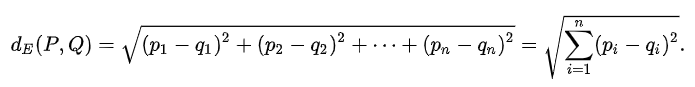
\includegraphics{capitulo2/images/distanciaEuclidiana.png}
			\caption{Fórmula para calcular la distancia Euclidiana.}
			\label{fig:distanciaEuclidiana2}
		\end{center}
	\end{figure} 
Para el caso del ejemplo se tendría el siguiente cálculo:
	\begin{figure}[H]
		\begin{center}
			\hypertarget{fig:distanciaejemplo}{\hspace{1pt}}
			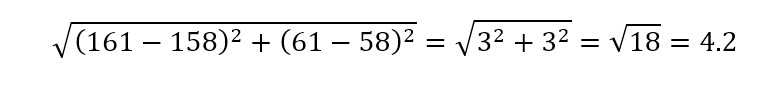
\includegraphics[width=.7\textwidth]{capitulo4a/images/distanciaejemplo.jpeg}
			\caption{Fórmula para calcular la distancia Euclidiana del ejemplo.}
			\label{fig:distanciaejemplo}
		\end{center}
	\end{figure}
Al momento de tener los cálculos de distancia se puede decir que se termina la intervención de la función Map en este algoritmo y se pasa la ejecución a la sección Reduce para que esta continué calculando los resultados de salida.
\\
\textbf{Función Reduce}: 
\\En esta función se recibe cada una de las lineas que se mandan desde el Map, y se hace un análisis de si este valor ya había sido recibido anteriormente, esto con el objetivo de que en caso de recibir valores duplicados estos sean manejados como un solo elemento y sólo se lleve un conteo que indique el número de veces que este elemento se ha repetido.
\\
Debido a que particularmente en este ejemplo no se tienen elementos duplicados esta funcionalidad no será evidente y no podrá ser demostrada, sin embargo, en la figura \ref{fig:fuknn} se muestra esta funcionalidad y se puede visualizar entre los pasos \emph{Mapeo} y \emph{Partición Intermedia} cómo se integran los datos repetidos y se presentan como un solo resultado con un número 2 asociado a él, lo cual indica que se trata de de un elemento que se repite 2 veces. 
\\
Primeramente, se arroja el archivo de salidas de manera desordenada es decir en el orden en el que se encuentran los renglones en el archivo de entradas. Esta tabla puede verse como se muestra a continuación:
\begin{table}[H]
		\begin{center}
			\label{tab:tablaKNNDistancias3}
			\begin{tabular}{c|c|c|c}
				\textbf{Altura (cm)} & \textbf{Peso (kg)} & \textbf{Talla} & \textbf{Distancia}\\
				\hline
				158 & 58 & M & 4.2\\
				158 & 59 & M & 3.6\\
				158 & 63 & M & 3.6\\
				160 & 59 & M & 2.2\\
				160 & 60 & M & 1.4\\
				163 & 60 & M & 2.2\\
				163 & 61 & M & 2.0\\
				160 & 64 & L & 3.2\\
				163 & 64 & L & 3.6\\
				165 & 61 & L & 4.0\\
				165 & 62 & L & 4.1\\
				165 & 65 & L & 5.7\\
				168 & 62 & L & 7.1\\
				168 & 63 & L & 7.3\\
				168 & 66 & L & 8.6\\
				170 & 63 & L & 9.2\\
				170 & 64 & L & 9.5\\
				170 & 68 & L & 11.4\\
			\end{tabular}
		\end{center}
		\caption{Tabla de salida no ordenada de Reduce}
	\end{table}
Mas adelante, la función Reduce también ordena todos los resultados obtenidos para todas las lineas entregadas por Map. en orden ascendente, es decir, se estaría generando la siguiente tabla.
	\begin{table}[H]
		\begin{center}
			\label{tab:tablaKNNDistancias}
			\begin{tabular}{c|c|c|c}
				\textbf{Altura (cm)} & \textbf{Peso (kg)} & \textbf{Talla} & \textbf{Distancia}\\
				\hline
				160 & 60 & M & 1.4\\
				163 & 61 & M & 2.0\\
				160 & 59 & M & 2.2\\
				163 & 60 & M & 2.2\\
				160 & 64 & L & 3.2\\
				158 & 59 & M & 3.6\\
				158 & 63 & M & 3.6\\
				163 & 64 & L & 3.6\\
				165 & 61 & L & 4.0\\
				165 & 62 & L & 4.1\\
				158 & 58 & M & 4.2\\
				165 & 65 & L & 5.7\\
				168 & 62 & L & 7.1\\
				168 & 63 & L & 7.3\\
				168 & 66 & L & 8.6\\
				170 & 63 & L & 9.2\\
				170 & 64 & L & 9.5\\
				170 & 68 & L & 11.4\\
			\end{tabular}
		\end{center}
		\caption{Tabla del conjunto de entrenamiento con la columna distancia ya calculada y ordenada.}
	\end{table}  
Sabiendo el valor del número K, el Reduce toma los primeros K elementos de esta tabla, suponiendo que:
K=5
Se generaría la siguiente tabla:
	\begin{table}[H]
		\begin{center}
			\label{tab:tablaKNNDistanciask}
			\begin{tabular}{c|c|c|c}
				\textbf{Altura (cm)} & \textbf{Peso (kg)} & \textbf{Talla} & \textbf{Distancia}\\
				\hline
				160 & 60 & M & 1.4\\
				163 & 61 & M & 2.0\\
				160 & 59 & M & 2.2\\
				163 & 60 & M & 2.2\\
				160 & 64 & L & 3.2\\
			\end{tabular}
		\end{center}
		\caption{Tabla del conjunto de entrenamiento con la columna distancias ya calculada para K=5}
	\end{table}
Posteriormente, se procede a intentar clasificar estos elementos dentro de una clase.\\
Para este ejemplo en particular se considerará la columna \emph{Talla} como la clase tomando esta clase como referencia para los 5 k nodos obtenidos se sabe que existen en el conjunto de k nodos:
\begin{itemize}
	\item 4 Elementos tipo M
	\item 1 Elemento tipo L 
\end{itemize}
Finalmente podrían arrojarse los 5 K nodos encontrados y con ellos mencionar que se puede clasificar como un elemento de tipo M, ya que existen más nodos encontrados de tipo M que de tipo L.
\\
Esta vendría siendo la salida final del algoritmo KNN, arrojando como salida los K elementos más cercanos encontrados y la clasificación encontrada para estos elementos. 
\newpage
\subsubsection{Diagrama de Flujo}
Se elaboro un diagrama de flujo que pretende modelar el funcionamiento de este algoritmo como lo hace en el paradigma MapReduce. 
El diagrama de flujo generado es el siguiente:
	\begin{figure}[H]
		\begin{center}
			\hypertarget{fig:diagramaflujo}{\hspace{1pt}}
			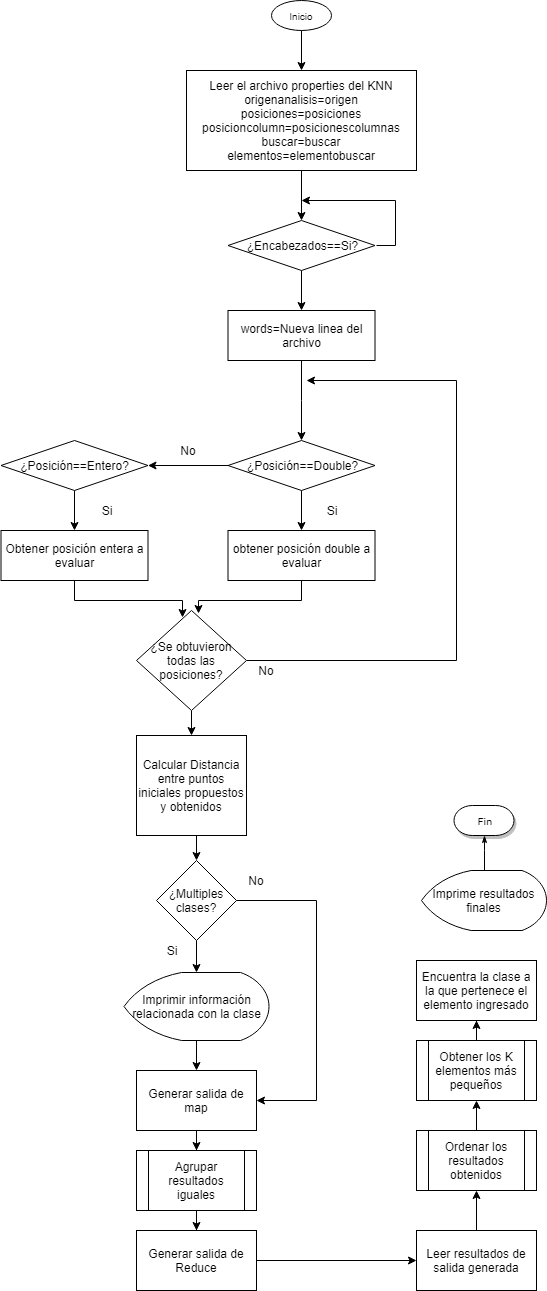
\includegraphics[width=.5\textwidth]{capitulo4a/images/KNN.png}
			\caption{Diagrama de Flujo para el algoritmo KNN.}
			\label{fig:diagramaflujo}
		\end{center}
	\end{figure}
Del diagrama de flujo presentado, se procede a explicar sus pasos:
\\
\begin{enumerate}
	\item Se lee el archivo "Properties" el cual almacena la información de los parámetros de configuración que requiere este algoritmo para empezar a funcionar, es decir:
	\begin{itemize}
		\item posicionescolumnas: Es el listado de posiciones dentro del archivo donde se encuentran los elementos que conforman la clase a buscar para que los K que se encuentren puedan ser agrupados en clases.\\ 
		\item Buscar: Se trata de una bandera la cual sirve para agregar un elemento en particular que se quiera buscar es decir, de todas las columnas que conforman las clases, se quiere buscar una clase en particular y centrarse únicamente en estos elementos. \\
		Cuando esta bandera se habilita, se tiene este comportamiento, sin embargo, mientras esta bandera no se habilite se consideran todos los elementos del archivo para el análisis.\\
		\item Elemento a buscar: Cuando la bandera \emph{Buscar} se habilita, es necesario especificar el elemento que conforma la clase particular a buscar. \\
		Esto se hace dando un elemento de cada una de las columnas especificadas en \emph{posicionescolumnas} de los cuales se desea realizar la búsqueda.\\
		\item Origen: Contiene los datos de referencia que se quieren buscar. Podría decirse que se trata de la nueva entrada de conocimiento, estos tienen que ser del mismo tipo de dato que las columnas de interés del usuario ademas de que deben de encontrarse en el mismo orden en que aparecen en el archivo.
		\\
		\item posiciones: Es el listado de los números de columnas que contienen la información que se desea tomar en cuenta para el análisis KNN de la totalidad del archivo.\\
		El resto de columnas que contenga el archivo y que no se encuentren listadas en esta sección simplemente serían ignoradas durante el proceso de análisis. 
		\\
		Es importante considerar que las columnas que se escojan para el análisis sean de tipo Double o Entero ya que en caso de no serlo, la ejecución de este algoritmo fallaría.
		\\
		\item K: es el número de k vecinos que se solicita encontrar para esta prueba   
	\end{itemize}
	\item El programa valida si se trata de un archivo que contenga encabezados o no, en caso de contenerlos, se omite una linea de lectura para no tomarlos en cuenta para el análisis y continuar con la siguiente.
	\item Cada que se lee una linea de datos valida se proceden a realizar lo siguiente:
	\begin{itemize}
		\item Se revisa que de los datos de la linea que se van a considerar para el análisis todos ellos sean del tipo de dato esperado y en caso de serlo, se obtiene su valor; en caso de no serlo, para al menos uno de ellos se omite la evaluación de esa linea.
		\item Cuando se tienen todas las posiciones, se calcula la distancia que existe entre el elemento a evaluar con el elemento obtenido en la entrada del archivo. 
		\item en caso de encontrarse que la linea leída no es un resultado concluyente ya que pertenece a múltiples clases se imprime la información obtenida para estas múltiples clases, en caso contrario simplemente se arroja la salida
		\item se compara la salida con salidas otorgadas anteriormente para comprobar que no se trate de una salida repetida ya que en caso de serlo se tiene que integrar a la contabilización de esa salida y no ser tratada como una nueva.
	\end{itemize} 
	\item Cuando se tienen todas las salidas es decir, cuando se terminó de leer el archivo, se procede a ordenarlas de la menor distancia a la mayor distancia.
	\item Teniendo esta información ya se puede conocer cuáles conforman los K vecinos mas cercanos y con ello otorgar el resultado final.
\end{enumerate}
\subsection{Algoritmo ID3}
Cada algoritmo MapReduce comienza su trabajo iniciando la actividad de un Job cada Job ejecuta las 5 tareas de el paradigma MapReduce, que como se sabe, solo se permite al programador tener injerencia en 2 de ellas sin embargo, una vez ejecutándose las 5 tareas se finaliza el programa. 
\\
En el caso particular del algoritmo ID3 se trata de un algoritmo que por definición se trata de un algoritmo recursivo.
Existen varias consideraciones a tomar en cuenta estas consideraciones se listan a continuación, a su vez como último punto listado se presenta la solución encontrada e implementada tomando en cuenta las consideraciones anteriores listadas en los puntos previos:
\begin{itemize}
	\item La forma de ejecución de un algoritmo basado en este paradigma consiste en realizar una ejecución particionada del archivo, esta partición es definida por el programador dentro de dicho algoritmo, pero sin importar el criterio de partición que se seleccione definitivamente no se puede realizar un tratamento de todos los datos en una sola exhibición por lo que se requiere procesar estas entradas de manera independiente una a una por la función Map.\\
	Posteriormente, la función Reduce puede hacer algunas operaciones con las salidas, sin embargo no puede regresar a ejecutar nuevamente la función map. \\
	Esto provocaría que se complicaran las cosas ya que al tratarse de un algoritmo recursivo es indispensable que este pueda repetir todos sus pasos cada vez que se manda a llamar, por lo que esta particularidad no haría posible ejecutar este algoritmo de manera inmediata.\\ 
	\item Otra propuesta fue iniciar un nuevo job cada vez que se requiriera de una llamada recursiva. Al intentar esto, ocurrió un problema ya que cada trabajo era independiente del trabajo anterior, por lo que los trabajos comenzaban a ejecutarse de manera paralela provocando que las ejecuciones se efectuarán de forma desincronizada y en ocasiones no fuera posible acceder a los resultados de trabajos que tenian que haber sido ejecutados antes, inclusive, se interrumpían las ejecuciones entre sí.
	\item Una tercera propuesta fue controlar la ejecución de cada uno de estos job de tal forma que no se comenzará la ejecución de uno nuevo hasta que el anterior no hubiera terminado, en ese sentido, se ejecuta cada uno de los trabajos de manera secuencial y no se interrumpen en sus tareas. \\
	Lo cual proporciona los resultados esperados, con esto se logro emular la funcionalidad de una operación recursiva pero desde la función principal del programa y no directamente dentro del código MapReduce. \\	
\end{itemize}
En el entendido de que cada MapReduce inicia un nuevo job se explicará el diseño que se realizo dentro de cada una de las funciones involucradas primero se hará para la función map, posteriormente se procederá a explicar la operación de la función reduce y por último se explicará cómo se hace uso de la recursividad desde la función principal.
\\
Para ello se tomará en cuenta el ejemplo mostrado en la sección \nameref{ejecucionID3} del marco teórico.\\
\textbf{Función Map}:
\\
La función Map en este algoritmo buscará primeramente tomar el listado de entradas y almacenarlas de una manera que sea sencilla de entender. \\
Para ser manipulada posteriormente, se convertirá el archivo de entradas con una estructura plana en una estructura, como la que se muestra a continuación:
\\
\begin{figure}[H]
	\begin{center}
		\hypertarget{fig:tablaID3}{\hspace{1pt}}
		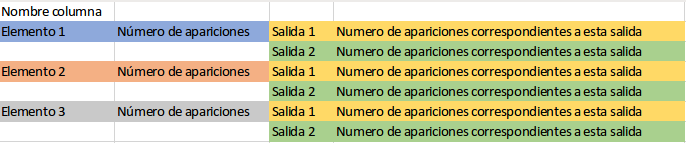
\includegraphics[width=.9\textwidth]{capitulo4a/images/tablaid3sinvalores.png}
		\caption{Tabla construcción ID3 sin valores.}
		\label{fig:tablaID3}
	\end{center}
\end{figure}
Donde se almacena:\\
-Para cada una de las columnas incluidas en el archivo de entradas de el algoritmo ID3 un listado de los elementos diferentes que la conforman.\\
-Para cada elemento se incluye el número de veces que este elemento aparece en el archivo de entradas.\\
De la totalidad de entradas encontradas se contabiliza cuántas de ellas pertenecen a la primera clase, y cuántas a la segunda clase.\\
La figura \ref{fig:tablaID32} muestra la estructura descrita con datos reales del ejemplo que se está revisando.
\begin{figure}[H]
	\begin{center}
		\hypertarget{fig:tablaID32}{\hspace{1pt}}
		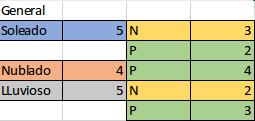
\includegraphics[width=.5\textwidth]{capitulo4a/images/tablaid3.png}
		\caption{Tabla construcción ID3 con valores de la columna Soleado.}
		\label{fig:tablaID32}
	\end{center}
\end{figure}
Esta tabla se va a actualizando cada vez que la función Map lee una nueva linea del archivo y al finalizar la lectura de todas las lineas se tiene una sola estructura que almacena la información de toda la tabla y que se fue refrescando a cada iteración. Por lo que se puede decir que los datos que en esta tabla se almacenan no son confiables hasta que se recorre el archivo de entradas en su totalidad, en otras palabras, al terminar la ejecución de la función Map.\\
Una vez que esta tabla es construida en su totalidad, se procede al tratamiento de la misma. \\
La cual se hace haciendo el cálculo de la entropía general de la tabla de entradas esto se hace tomando los valores de la columna de salidas. \\
Luego de la entropía específica de cada uno de los diferentes elementos que se encuentran en cada columna.\\
Con el cálculo de estos valores se procede a realizar el cálculo de la entropia general de cada fila y posteriormente con este valor encontrar la ganancia correspondiente a cada fila. \\
La ganancia mayor calculada con todas las filas, será la que se tome en cuenta para llevar a cabo la siguiente iteración.\\
La forma en que se hacen estos cálculos es la misma manera que como se hace tradicionalmente se puede saber esto consultando la sección \nameref{ejecucionID3}.\\ 
Una parte importante que mencionar es que si resulta que todos los elementos que se están evaluando terminan en un mismo resultado de salidas, eso significa que no se requiere realizar más evaluaciones, por lo que se llego a un resultado final. En este caso no se realizan los cálculos de entropía y ganancia mencionados en los párrafos anteriores y en su lugar se devuelve un fin de recursión, esto buscando que la recursividad se detenga.\\
\textbf{Función Reduce}: 
\\
La función \emph{Reduce} en este problema sirve para presentar los resultados calculados en el map y agruparlos de tal forma que puedan ser claramente presentados. \\
Por otro lado también permite preparar la siguiente corrida del algoritmo en caso de que requiera aplicar la recursividad.\\
\textbf{Función Principal}
Se considera que esta es la parte mas importante a tomar en cuenta para comprender cómo es que funciona esta implementación por lo que esta parte se procederá a explicar a detalle.
\\
\textbf{La funcion Main}: Únicamente obtiene las dimensiones del archivo buscando conocer el número de columnas.\\
Posteriormente invoca a la función recursiva que es la que hace todo el trabajo. La cual se explicará mas adelante una vez que la función recursiva termina se escribe el resultado final obtenido durante toda la ejecución del algoritmo en el archivo de salida.\\
\textbf{La función Recursiva}:\\
esta función tiene una estructura que de manera simplificada se puede escribir como sigue:
 \begin{verbatim}
Función recursiva:
   Número_de_iteraciones=numero_de_palabras:
        Se escriben resultados
        Termina iteracion por exceso de intentos y porque ya se probo con todas las columnas
   Se_llego_a_caso_base:
        Se escriben resultados
        Termina iteración por llegar a solución 
   Ninguno_de_los_anteriores:
        Se crea subtabla
        Se invoca nuevamente a funcion recursiva
 \end{verbatim}
Como se puede ver, se tienen 3 condiciones, dos de ellas son condiciones de paro y la tercera es una condición de recursividad. A continuación se realiza la evaluación de lo que hace cada una de ellas. 
	\\
El algoritmo busca establecer las condiciones que se tienen que tomar en cuenta para hacer una clasificación, por lo tanto, cuando tiene todas estas condiciones completas el algoritmo termina. 
	\\
No sin antes escribir los resultados encontrados, es decir, que columnas se tienen que tomar en cuenta para llevar a cabo esta clasificación.
	\\ 
\begin{itemize}
	\item Condición de paro 1:
	Cuando se encuentra que todos los elementos contenidos en la columna correspondiente a las clases son iguales significa que el elemento ha sido clasificado.\\
	En este caso en particular no es necesario realizar nuevamente el cálculo de las entropias y las ganancias, por lo que solo es necesario establecer que se trata de un caso base, esto se hace indicando que la siguiente columna a evaluar es -1 y cuando se encuentra este resultado únicamente se detienen las invocaciones a la funcion recursiva para la tabla que se esta evaluando.\\
	\item Condición de paro 2: \\
	Cuando el contador de iteraciones llega a ser igual al numero de columnas contenidas en el archivo significa que ya fueron evaluadas todas las columnas posibles y con ello todos los datos disponibles han sido tomandos en cuenta.\\
	En este caso se tiene una tabla de solo un renglón ya que para este punto se han descartado todas las columnas. y al tratarse de una sola posibilidad a pesar de no haberse podido simplificar su clasificación.\\ 
	El renglón esta clasificado para el peor posible caso. En esta situación se escribe la clasificación a la que se llego y se detienen las llamadas recursivas.\\
	\item Condición de recursividad: Cuando ninguna de las 2 anteriores se cumple significa que no se ha logrado llegar a una solución por lo que es necesario seguir iterando.\\
	Esto quiere decir que se volverá a invocar a otro job que ejecute nuevamente las tareas MapReduce. únicamente cambiando la tabla de entradas. e incrementando el número de veces que se ha realizado la recursividad, esta segunda con el objetivo de llevar un control de la primer condición de paro la cual controla el número de iteraciones. \\ 
\end{itemize}
\textbf{Subtabla}: Esta función permite crear tablas más pequeñas de acuerdo a los resultados obtenidos durante el análisis, para que estas nuevas tablas sean las que se manden a evaluar en la siguiente iteración de MapReduce.
Por ejemplo, para el caso de la tabla de entradas vista en el marco teórico que se muestra a continuación:
\\
\begin{table}[!hb]
	\begin{center}
		\label{tab:tablaInduccionID3}
		\begin{tabular}{c|c|c|c|c|c}
			\textbf{Día} & \textbf{Aspecto} & \textbf{Temperatura} & \textbf{Humedad} & \textbf{Viento} & \textbf{Decisión}\\
			\hline
			1 & Soleado & Caluroso & Alta & Ligero & No\\
			2 & Soleado & Caluroso & Alta & Fuerte & No\\
			3 & Nublado & Caluroso & Alta & Ligero & Sí\\
			4 & Lluvioso & Templado & Alta & Ligero & Sí\\
			5 & Lluvioso & Fresco & Normal & Ligero & Sí\\
			6 & Lluvioso & Fresco & Normal & Fuerte & No\\
			7 & Nublado & Fresco & Normal & Fuerte & Sí\\
			8 & Soleado & Templado & Alta & Ligero & No\\
			9 & Soleado & Fresco & Normal & Ligero & Sí\\
			10 & Lluvioso & Templado & Normal & Ligero & Sí\\
			11 & Soleado & Templado & Normal & Fuerte & Sí\\
			12 & Nublado & Templado & Alta & Fuerte & Sí\\
			13 & Nublado & Caluroso & Normal & Ligero & Sí\\
			14 & Lluvioso & Templado & Alta & Fuerte & No\\
		\end{tabular}
	\end{center}
	\caption{Tabla de inducción para juegos de tenis ID3.}
\end{table}
y posterior de eso, después de el primer cálculo se detecta que la mayor ganancia se encuentra en la columna \textbf{Aspecto}. por lo que en este caso, existen 3 valores diferentes en esta columna:\\
-Soleado\\
-Nublado\\
-Lluvioso\\
Esta función entonces tendría que crear las siguientes 3 subtablas para mandarlas a ejecución, en el siguiente ciclo, las cuales serian:\\
\begin{table}[H]
	\begin{center}
		\label{tab:tablaInduccionID3}
		\begin{tabular}{c|c|c|c|c|c}
			\textbf{Día} & \textbf{Aspecto} & \textbf{Temperatura} & \textbf{Humedad} & \textbf{Viento} & \textbf{Decisión}\\
			\hline
			1 & Soleado & Caluroso & Alta & Ligero & No\\
			2 & Soleado & Caluroso & Alta & Fuerte & No\\
			8 & Soleado & Templado & Alta & Ligero & No\\
			9 & Soleado & Fresco & Normal & Ligero & Sí\\
			11 & Soleado & Templado & Normal & Fuerte & Sí\\
		\end{tabular}
	\end{center}
	\caption{Tabla 1.}
\end{table}
\begin{table}[H]
	\begin{center}
		\label{tab:tablaInduccionID3}
		\begin{tabular}{c|c|c|c|c|c}
			\textbf{Día} & \textbf{Aspecto} & \textbf{Temperatura} & \textbf{Humedad} & \textbf{Viento} & \textbf{Decisión}\\
			\hline
			3 & Nublado & Caluroso & Alta & Ligero & Sí\\
			7 & Nublado & Fresco & Normal & Fuerte & Sí\\
			12 & Nublado & Templado & Alta & Fuerte & Sí\\
			13 & Nublado & Caluroso & Normal & Ligero & Sí\\
		\end{tabular}
	\end{center}
	\caption{Tabla 2}
\end{table}
\begin{table}[H]
	\begin{center}
		\label{tab:tablaInduccionID3}
		\begin{tabular}{c|c|c|c|c|c}
			\textbf{Día} & \textbf{Aspecto} & \textbf{Temperatura} & \textbf{Humedad} & \textbf{Viento} & \textbf{Decisión}\\
			\hline
			4 & Lluvioso & Templado & Alta & Ligero & Sí\\
			5 & Lluvioso & Fresco & Normal & Ligero & Sí\\
			6 & Lluvioso & Fresco & Normal & Fuerte & No\\
			10 & Lluvioso & Templado & Normal & Ligero & Sí\\
			14 & Lluvioso & Templado & Alta & Fuerte & No\\
		\end{tabular}
	\end{center}
	\caption{Tabla 3}
\end{table}
Como se puede ver, lo que hace esta función es crear las tablas para cada uno de los valores contenidos en la columna que posee la mayor ganancia una vez que la tabla ha sido construida se vuelve a invocar a MapReduce las veces que sean necesario y las funciones recursiva junto con subtabla se encargan de la administración de las llamadas recursivas.
\subsubsection{Diagrama de Flujo}
Se elaboró el siguiente diagrama de flujo el cual pretende modelar el funcionamiento del algoritmo ID3 como se hace en el paradigma MapReduce, el diagrama de flujo generado es el siguiente:
\\
\begin{figure}[H]
	\begin{center}
		\hypertarget{fig:flujo}{\hspace{1pt}}
		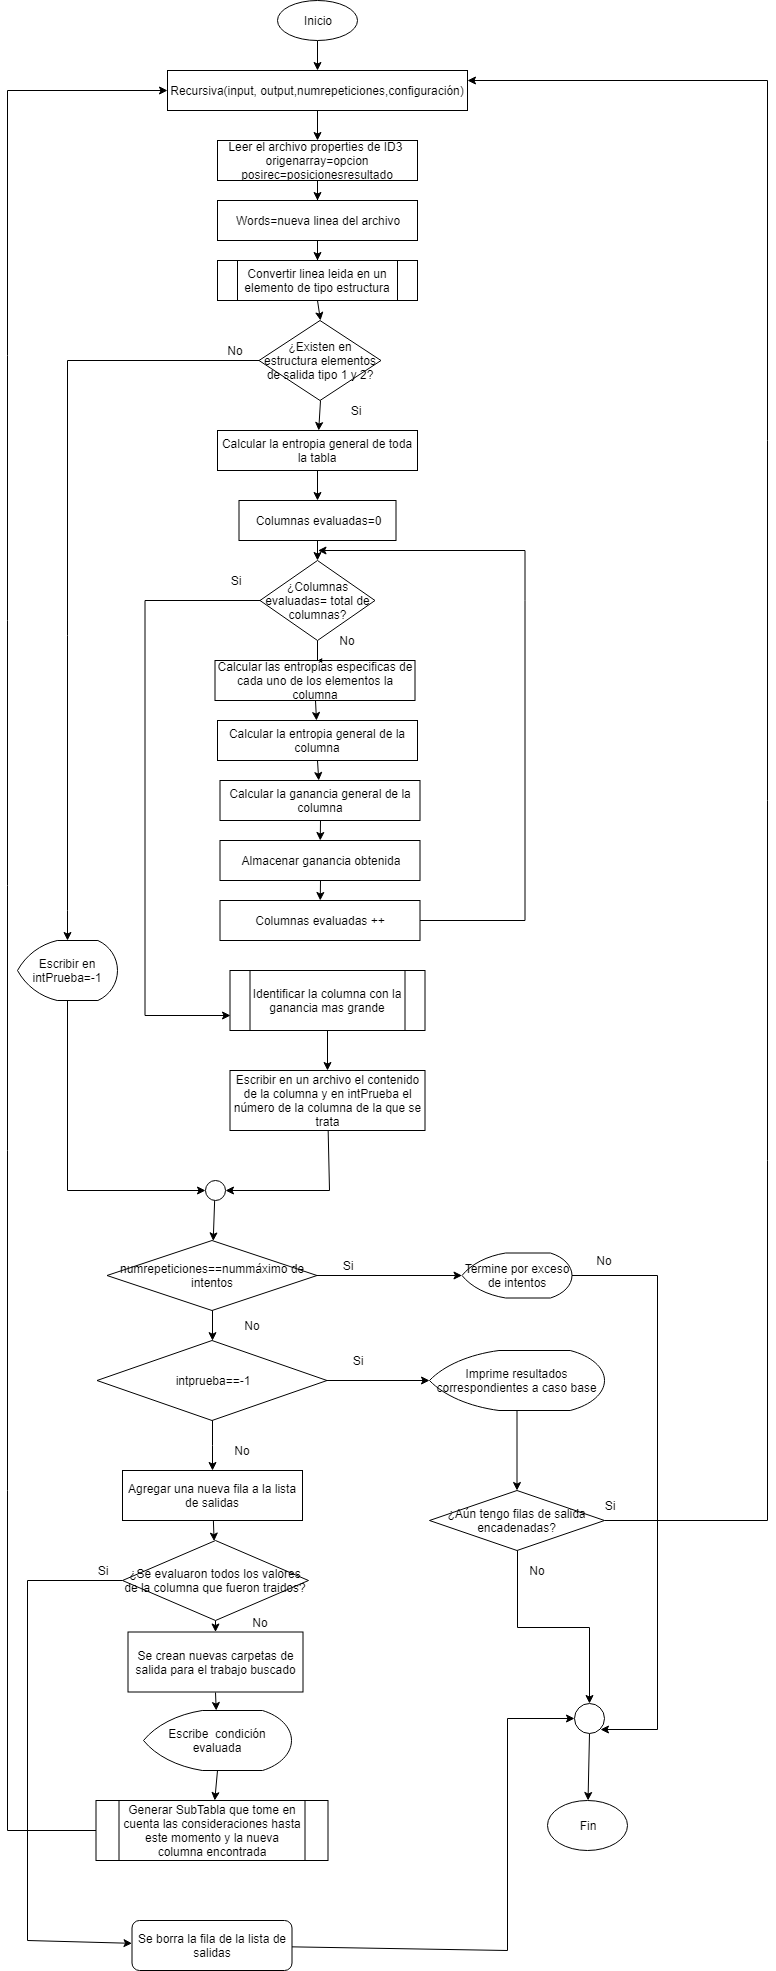
\includegraphics[width=.55\textwidth]{capitulo4a/images/ID3.png}
		\caption{Funcionamiento completo de algoritmo KNN con todas sus operaciones en Hadoop.}
		\label{fig:flujo}
	\end{center}
\end{figure}
Del diagrama de flujo presentado, se procede a explicar sus pasos:
\begin{enumerate}
	\item El primer paso, es la invocación de la función recursiva para que este ejecute en el primer caso para la tabla original y en lo subsecuente para las tablas generadas.
	\item Se lee el archivo "Properties" el cual almacena la información de los parámetros de configuración que requiere este algoritmo para funcionar:
	\begin{itemize}
		\item origenarray: contiene las opciones de resultados que se pueden presentar durante la ejecución del algoritmo.\\ 
		En otras palabras se trata de el conjunto de opciones de salida que se tienen. \\
		únicamente pueden ser 2 ya que se trata de un algoritmo de salida de tipo binario y vienen separadas por comas.
		\item posirec: Contiene la posición en el archivo en la que se encuentran los resultados. Es un elemento de tipo numérico y empieza a contar de 0 en adelante.
	\end{itemize}
	\item Se lee una nueva linea el archivo que contiene la tabla para comenzar a trabajar con ella.
	\item Para la linea leída se hace el tratamiento correspondiente para que se convierta en un elemento de tipo estructura como el que se explicaba anteriormente, esto con la finalidad de facilitar su tratamiento.
	\item Se valida que la estructura tenga 2 diferentes tipos de salida, es decir, que esta no haya sido clasificada aún.
	Si se encuentra que se trata de un elemento ya clasificado. entonces se indica que no hay ninguna nueva columna a evaluar esto asignándole al valor de la nueva columna a evaluar -1 y con esto, haciendo posible que la función recursiva se detenga en este punto.\\
	En caso de que aun no se haya llegado a la solución, entonces se procede a realizar todos los cálculos que se enlistan en los siguientes puntos.
	\item Lo primero es calcular la entropia, general de toda la tabla. 
	\item Posteriormente, se va columna por columna en la tabla, calculando las entropias de cada elemento en cada una de las columnas.
	\item Teniendo todas las entropias correspondientes a una columna, se calcula la entropia general de la columna.
	\item Una vez teniendo la entropia general de la columna con ella se puede calcular la ganancia de esta columna.
	\item Cuando se tienen todas las entropias y ganancias correspondientes, es necesario comparar todas las ganancias de columnas obtenidas.\\
	Con el fin de obtener la mas grande y conservarla como la columna sobre la que se van a ejecutar los cálculos.
	\\
	Cuando se conoce esta columna se procede a establecer en un archivo todos los elementos contenidos dentro de la columna y establecer el numero de la columna de la que se trata.
	\item Cuando se hace esto entonces se vuelve a la función recursiva y se realizan las validaciones correspondientes.\\
	\begin{itemize}
		\item En el caso de que se haya alcanzado el numero máximo de intentos, es decir, la condición 1 entonces se establece esto como salida, se escribe el resultado obtenido y se rompe la ejecución de la función recursiva.\\
		\item En caso de que se trate de un caso base sera necesario escribir el resultado obtenido para posteriormente romper la ejecución de la función recursiva.\\
		\item En caso de que no sea ninguna de las anteriores, se procede a preparar la ejecución para que se haga nuevamente.
		\\Esto se hace tomando en cuenta que para cada columna se tiene mas de un elemento, entonces, cuando se ejecuta el ultimo de ellos, quiere decir que ya se termino la ejecución de esta columna, lo que que será necesario eliminarla de la lista de salidas.\\
		En caso de que no se trate de esta situación entonces se prepara el ambiente necesario para la ejecución de un nuevo job. esto se consigue destinando una nueva carpeta de salida, ya que, cada job requiere una independiente para su ejecución.
		\\
		Posteriormente, se escriben los resultados parciales obtenidos hasta este momento durante la ejecución del algoritmo.\\
		Y por ultimo es necesario generar la subtabla con la información recuperada de lo que debe contener la nueva tabla a ser ejecutada. 
	\end{itemize}
\end{enumerate}
\section{Desarrollo}
\subsection{Algoritmo KNN}
El algoritmo KNN escrito en JAVA servirá para realizar operaciones de clasificación sobre los datos que se almacenen en el HDFS por parte de los usuarios finales.
\\
Este algoritmo, al igual que todos los algoritmos que sean programados con el paradigma Map Reduce. únicamente se requiere programar sus secciones de Map y de Reduce, mientras que para el resto de secciones no contempladas este paradigma las auto completa para poder funcionar.
\\
Sin embargo para que esta funcionalidad pueda operar de manera correcta es necesario que se siga el paradigma de programación Map Reduce, ya que en caso de no hacerlo como se indica el resto de funciones intermedias no podrían integrarse como se espera.
\\
Se leerán y procesarán archivos de texto con formato CSV, entradas que permitirá el algoritmo. 
\\
Con lo que, este algoritmo podrá procesar archivos de datos que tengan una fila de datos de encabezado y al mismo tiempo podría hacerlo si este archivo no la tiene. \\
Para el correcto funcionamiento de este algoritmo se pueden hacer las siguientes consideraciones: 
\begin{itemize}
	\item Es importante invocar un algoritmo de ordenamiento que permita ordenar los resultados obtenidos, esto para obtener un método de ordenamiento optimo que permita optimizar la solución y como , se sabe que se trabajaría mayormente con grandes cantidades de datos, se busca que este algoritmo sea lo mas optimo posible.
	\item Es necesario realizar la importación de las librerías de Map y de Reduce, ya que, se trata de librerías requeridas por Hadoop para que este algoritmo pueda funcionar.
	\item Se utilizan archivos de salida adicionales para poder gestionar el resto de salidas y poder ver los resultados en diferentes puntos del proceso, lo cual podría tener gran valor para el usuario final. 
	\item Se agrego una salida en formato de datos de Excel esta con el objetivo de que el manejo de datos sea mas fácil para el usuario final, y se puedan utilizar las funcionalidad de Excel para manipular los resultados de salida.  
	\item Se permite personalizar desde el archivo de configuraciones las rutas donde el usuario desea escribir las salidas, para que este pueda tener control de las diferentes ejecución que haga y donde estas se están almacenando.
	\\
	\item En ocasiones los archivos de datos tienen registros repetidos que no vale la pena contabilizar como mas de un vecino, ya que se trata del mismo.en este caso se realiza una agrupación para que se consideren uno mismo y solamente se le notifica al usuario cuantas veces se encontró este vecino en particular a lo largo del archivo. 
\end{itemize}

En la imagen \nameref{fig:fuknn} se puede visualizar el funcionamiento completo que tendría que ejecutarse en el cluster para llevar a cabo este algoritmo.
	\begin{figure}[H]
		\begin{center}
			\hypertarget{fig:fuknn}{\hspace{1pt}}
			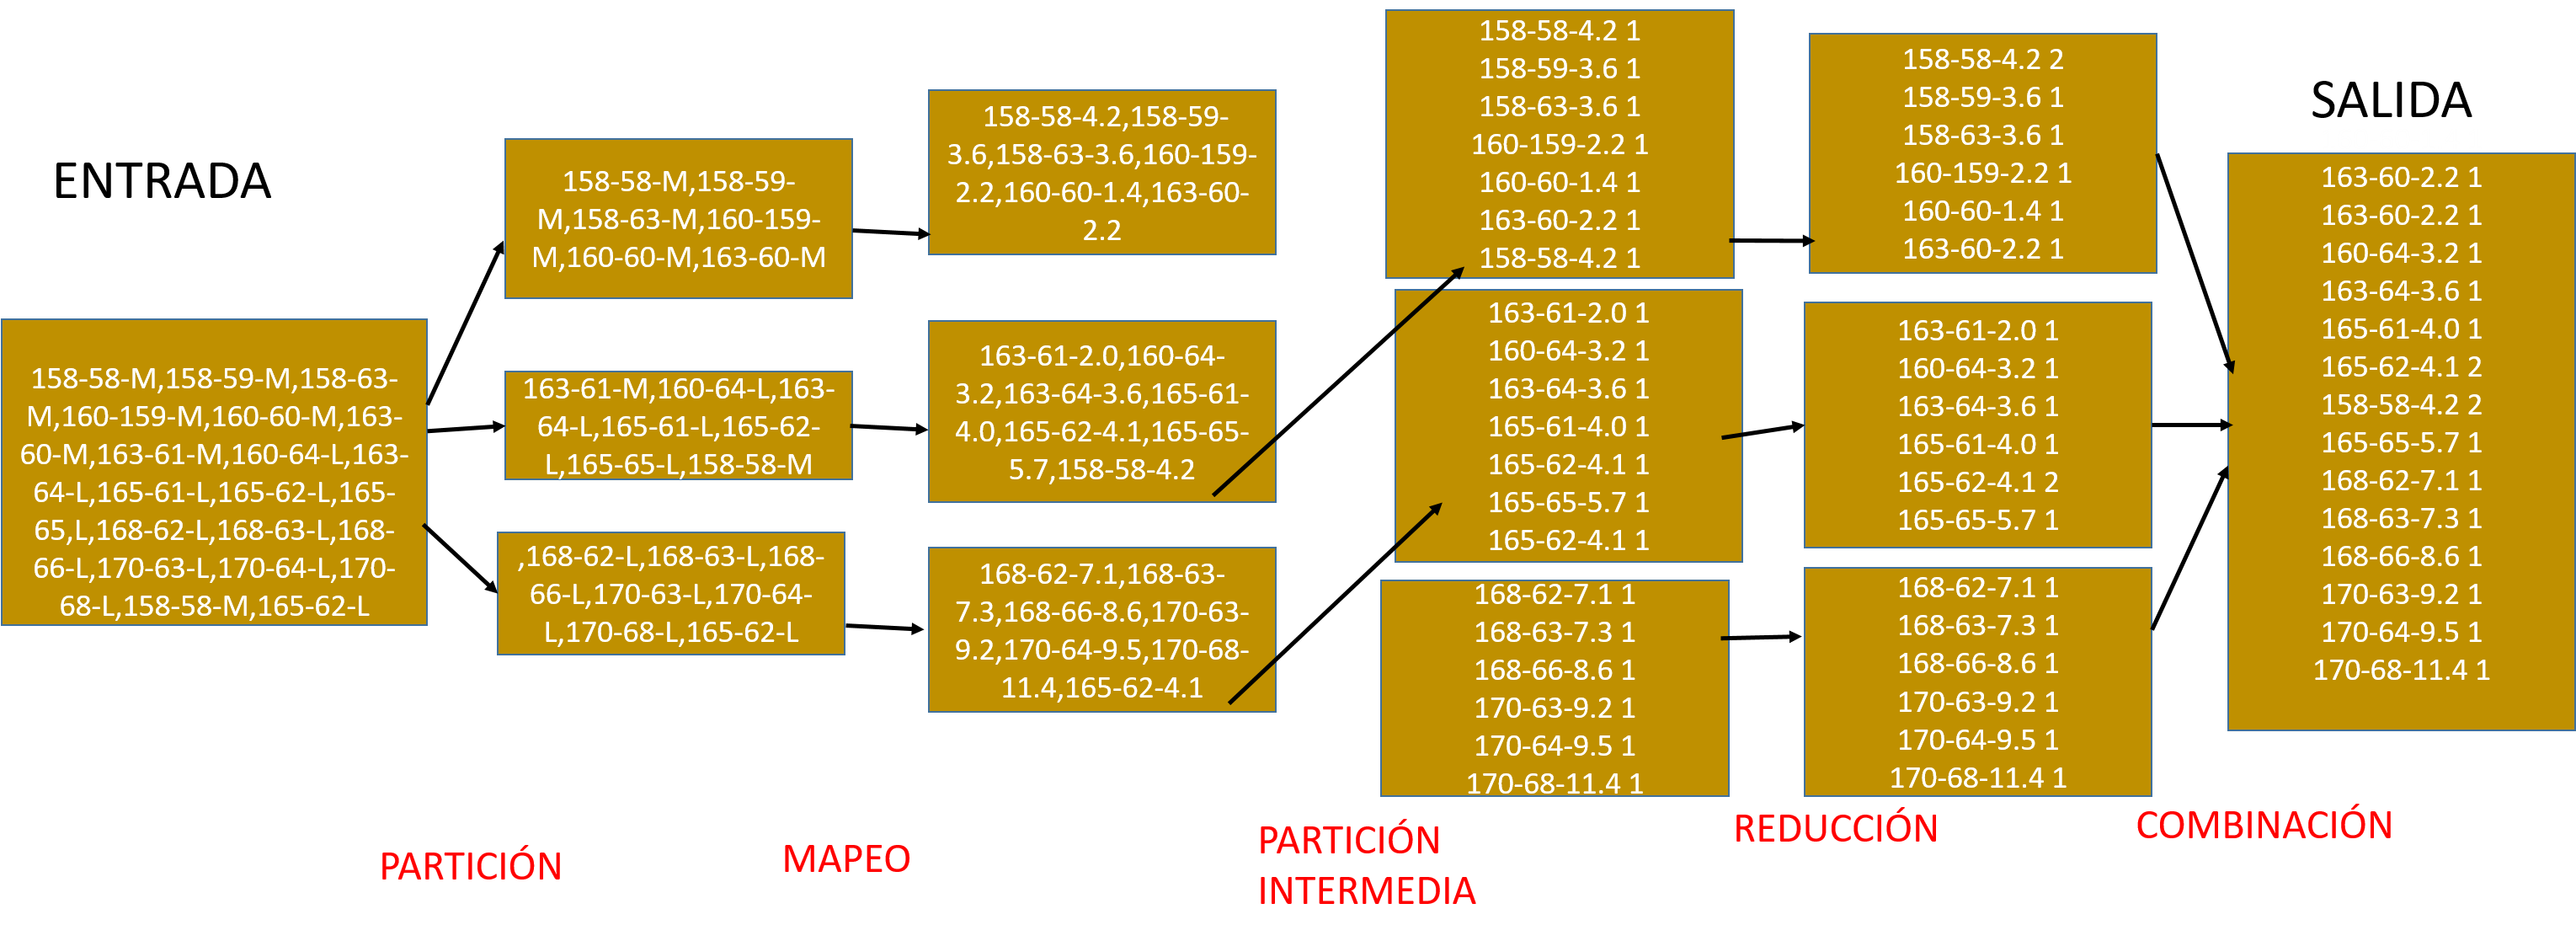
\includegraphics[width=.9\textwidth]{capitulo4a/images/ImagenKNN.png}
			\caption{Funcionamiento completo de algoritmo KNN con todas sus operaciones en Hadoop.}
			\label{fig:fuknn}
		\end{center}
	\end{figure}
Se explicarán los módulos que forman parte de la ejecución de el algoritmo KNN haciendo uso del paradigma MapReduce.
\begin{enumerate}
	\item \textbf{Partición}: Se requiere definir un parametro de partición, esto para que se puedan reconocer las unidades a analizar y con esto poder asignar tareas a los nodos. el parámetro de partición puede ser cualquier cosa, por ejemplo, dividir por espacio, coma, punto y coma, o incluso por una nueva línea ('\ n').
	En este caso, se realiza por una nueva línea del archivo es decir ('\ n').
	\item \textbf{Mapeo}: La explicación de esta parte ya se realizo anteriormente en la sección \nameref{seccionalgoritmomapreduce} 
	 \texttt{Función Map}.
	\item \textbf{Partición intermedia}:Se busca generar grupos con los datos que después de pasar por el módulo de mapeo y tener la estructura de salida de este modulo tienen la misma CLAVE, al cumplir esta condición se asignan en el mismo grupo. Se generan tantos grupos como claves existan.
	\item \textbf{Reducción}: Se explicó anteriormente en \nameref{seccionalgoritmomapreduce} \texttt{Función Reduce}. 
	\item \textbf{Combinación}: Todos los datos de salida que arrojó la función de reducción son combinados y puestos en un sólo grupo para generar un resultado final.
\end{enumerate}		
Es necesario generar un JAR para la ejecución de este algoritmo, esto se hace ya sea desde un IDE de Java, una instalación de Java en alguna de las maquinas, como la que efectúa el \nameref{cap:Cap5} o bien desde el mismo Hadoop, esto podría hacerse ejecutándose el siguiente comando:
 \begin{verbatim}
 	bin/hadoop com.sun.tools.javac.Main [clase_principal_java].java
 	jar cf [Nombre_jar].jar [clase_principal_java]*.class
 \end{verbatim}
\subsection{Algoritmo ID3}
El algoritmo ID3 escrito en Java permite realizar operaciones soportadas por los arboles de decisión sobre los datos que se almacenen en el HDFS por parte de los usuarios finales. \\
únicamente es necesario realizar la programación correspondiente a la sección Map y a la sección Reduce de acuerdo a las consideraciones de programación propuestas durante la sección de diseño. 
\\
A continuación se listan las consideraciones que se tienen que tomar en cuenta para el correcto funcionamiento de este algoritmo:
\begin{itemize}
 \item Este algoritmo soporta ejecuciones para cualquier entrada de datos en formato tabla siempre y cuando se cumpla la condición de que, la columna que se desee utilizar como columna de salida, solamente tenga 2 posibles opciones de resultado, lo cual permitiría hacer la clasificación de los elementos. \\
 \item Este algoritmo acepta archivos de tipo .txt y de tipo .csv es decir archivos de texto plano con la única obligatoriedad de que los separadores que existan entre las columnas que conforman el archivo sean \emph{,} coma. ya que dentro del código se utiliza este carácter como separador.\\
 \item Se requiere que la carpeta donde se van a escribir los resultados parciales a partir de la segunda ejecución no exista y en caso de existir que no contenga archivos propios de una ejecución anterior, ya que en caso de hacerlo este intentará sobre escribirlos y se generará un error en tiempo de ejecución.
 \item El archivo properties contiene las configuraciones de ordenes de ejecución para cambiar y manipular entre ejecución y ejecución. 
 \item Debido a que el programa levanta múltiples jobs para realizar un mismo trabajo, no hay una forma certera de conocer el progreso en la ejecución del algoritmo ya que el contado de Map y Reduce se estarán reiniciando cada que se levante un nuevo job. Por lo que, cuando ambos se vean muy cercanos al 100\% no es una señal de que el algoritmo está por terminar, sino mas bien que una de las ejecuciones esta por hacerlo.
\end{itemize}
Este algoritmo se programó haciendo además la implementación de una clase que se llama Estructura, la cual contiene la definición que representa a una entrada dentro del archivo para facilitar su tratamiento. \\
Esta clase es independiente de las clases que son utilizadas para la propia corrida del algoritmo, y es de utilidad ya que permite simplificar el manejo de los datos, en diferentes puntos del algoritmo.\\
Estructurarlos de una manera cómoda simplifica el tratamiento de los datos y puede hacer mas simple su manejo en diferentes puntos de la de la ejecución.\\
Por lo que respecta a lo propio del algoritmo se siguió lo estipulado en el diseño para el desarrollo del mismo , y se tiene una programación que empata por completo con el diseño que se propuso para su funcionamiento. \\
Para que el código fuente pueda ser funcional y pueda ser ejecutado desde Hadoop, es necesario que este se encuentre compilado como un JAR, para realizar esta tarea, es posible utilizar el siguiente comando. 
 \begin{verbatim}
 	bin/hadoop com.sun.tools.javac.Main [clase_principal_java].java
 	jar cf [Nombre_jar].jar [clase_principal_java]*.class
 \end{verbatim}
 Cuando se tenga al código fuente representado como un JAR, entonces se podrá ejecutar como se indica en la sección de pruebas para obtener los resultados esperados para los casos de prueba que tenga el usuario.
\section{Pruebas} \label{pruebasalgoritmos}
\subsection{Algoritmo KNN}
\subsubsection{Prueba 1}
A continuación se muestra una prueba de la ejecución de este algoritmo para comprobar su correcto funcionamiento y que esta operando como debería hacerlo:
\\
Para ello y con el objetivo de que sea mas claro, se utilizará el mismo ejemplo que se viene manejando durante todo el capitulo y también en el marco teórico. 
\\
Esto porque, es un ejemplo que ya se conoce y que facilitará el entendimiento de la prueba. 
\\
Como primer instancia es necesario crear el archivo de configuraciones para esta ejecución el cual, deberá contener la siguiente información:
\label{posiciones}
\begin{verbatim}
posicionescolumnas=1

buscar=N

elementoabuscar=

origen= 161,61

posiciones=1,2

K=5
\end{verbatim} 
Con esta configuración indicaremos:
\begin{enumerate}
 \item Se quiere agrupar tomando en cuenta el contenido de la columna 1 es decir la que contiene información relacionada con el peso
 \item No se desea buscar ningún elemento de peso en especifico por lo que se dice que no y no se indica en elemento a buscar.
 \item El elemento a tomar de referencia o bien, el que se quiere comparar esta representado por los valores 158, 58
 \item Las posiciones en el archivo que se desea utilizar para realizar esta evaluación son las posiciones 1 y 2 es decir las que contienen la Altura (cm) y el Peso en (kg).
 \item Se desea encontrar los 5 vecinos mas cercanos.
Por otro lado, otro archivo importante a construir antes de comenzar las pruebas es el archivo de entradas.
\\
Este archivo contiene la tabla con la información de entradas con la que se alimentará el algoritmo, para este ejemplo particular, el archivo tendrá el contenido siguiente: 
\begin{verbatim}
Altura,Peso,Talla
160,60,M
163,61,M
160,59,M
163,60,M
160,64,L
158,59,M
158,63,M
163,64,L
165,61,L
165,62,L
158,58,M
165,65,L
168,62,L
168,63,L
168,66,L
170,63,L 
170,64,L 
170,68,L 
\end{verbatim}
Una vez que se han creado estos 2 archivos es necesario que estos se suban al HDFS ya que serán necesarios en el momento que el algoritmo se ejecute.
\\
Para comenzar el proceso, primeramente se ejecuta el siguiente comando:
\begin{verbatim}
root@maestro:/opt/hadoop/etc/hadoop: yarn jar /home/mayra/Escritorio/MRProgramsDemo.jar 
PackageDemo.WordCount "user/luminus/documentoknn1/tabla.txt" "user/luminus/documentoknn1/output" 
"user/luminus/documentoknn1/configuracion.properties"
\end{verbatim} 
como puede visualizarse en la imagen siguiente.\\
\end{enumerate}
	\begin{figure}[H]
		\begin{center}
			\hypertarget{fig:funcio}{\hspace{1pt}}
			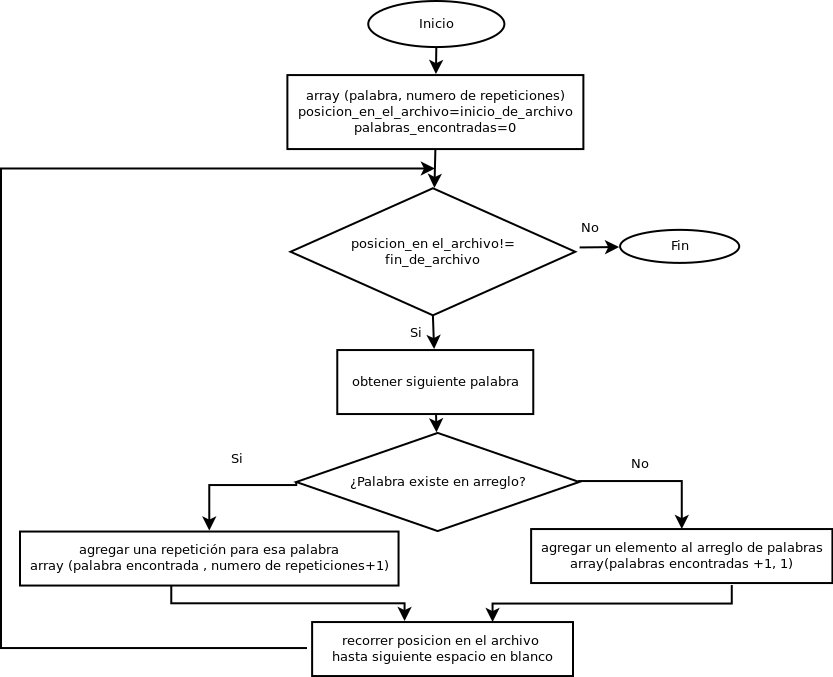
\includegraphics[width=.9\textwidth]{capitulo4a/images/im1.png}
			\caption{Funcionamiento completo de algoritmo KNN con todas sus operaciones en Hadoop.}
			\label{fig:funcio}
		\end{center}
	\end{figure}
Con esto empezará la ejecución del algoritmo y solo será cuestión de esperar a que se finalice su ejecución de manera correcta esto ocurre cuando el archivo termina de escribir todos los archivos correspondientes en el directorio como se muestra en la imagen \ref{fig:finknn1}
\begin{figure}[H]
	\begin{center}
		\hypertarget{fig:finknn1}{\hspace{1pt}}
		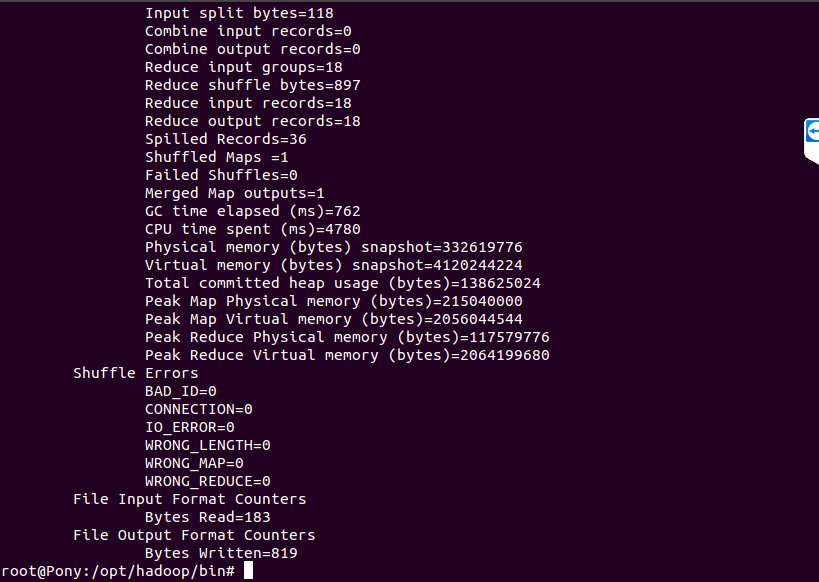
\includegraphics[width=.9\textwidth]{capitulo4a/images/corrida3.png}
		\caption{Termino de ejecución de algoritmo knn.}
		\label{fig:finknn1}
	\end{center}
\end{figure}
Cuando esta ejecución finalice, se podrán ver las salidas generadas por Hadoop directamente en el HDFS. se presenta una captura de pantalla de la información desplegada en el directorio indicado durante la ejecución en la figura \ref{fig:directorio}
\begin{figure}[H]
	\begin{center}
		\hypertarget{fig:directorio}{\hspace{1pt}}
		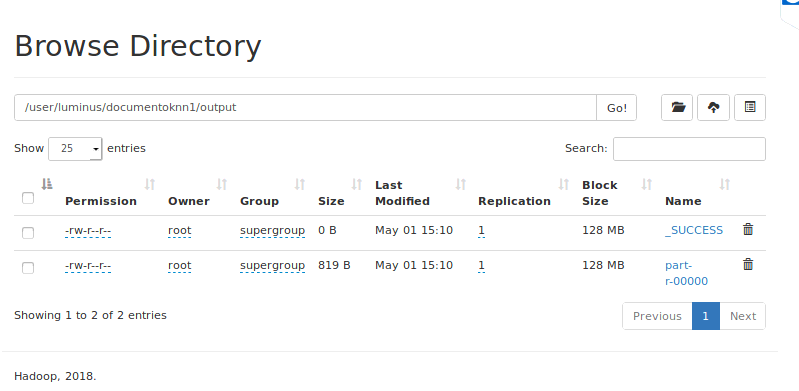
\includegraphics[width=.9\textwidth]{capitulo4a/images/corrida4.png}
		\caption{Directorio de salida del HDFS.}
		\label{fig:directorio}
	\end{center}
\end{figure}
como siguiente paso, se procede a visualizar el contenido del archivo llamado \emph{part-r-00000} el cual contiene la información de salida correspondiente a esta ejecución. El contenido de este archivo se muestra en la figura \ref{fig:contenido}
\begin{figure}[H]
	\begin{center}
		\hypertarget{fig:contenido}{\hspace{1pt}}
		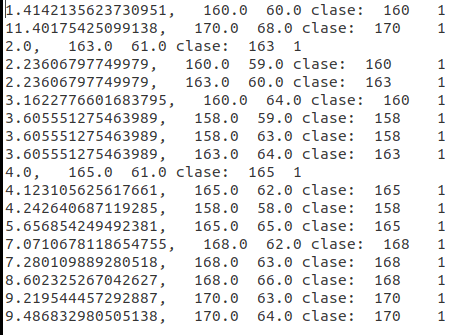
\includegraphics[width=.7\textwidth]{capitulo4a/images/corrida5.png}
		\caption{Archivo de salidas part-r-00000.}
		\label{fig:contenido}
	\end{center}
\end{figure}
Dentro de este archivo se puede visualizar el cálculo de distancias que se hizo para cada uno de los puntos dados, con respecto al punto.
\begin{lstlisting} 
	Altura (cm), Peso (Kg), Talla
	158 , 58 , M
\end{lstlisting} 
para cada uno de ellos se especifica:
\begin{itemize}
	\item El valor de distancia calculado entre cada uno de los puntos del archivo y el punto de referencia especificado.
	\item Los valores de Altura y Peso que se encontraron en cada renglón del archivo, que fueron utilizados en ese renglón especifico para hacer el cálculo de distancias 
	\item La clase a la que pertenece, ese elemento en particular, la cual puede ser escogida entre una o más columnas del archivo.
	En este caso se selecciono la clase Altura como se puede ver en el primer archivo de properties llenado, al inicio de la sección \nameref{posiciones}. Donde se especifica que posicionescolumnas=1 es decir que se tomará como referencia la columna 1 que corresponde a Altura.
	\item Un contador que indica el numero de veces que se repite cada elemento dentro del archivo, como en este caso todos son diferentes, cada uno de ellos viene etiquetado con el valor de 1.
\end{itemize}
Como se mencionaba anteriormente, esta solo representa la primera salida, ya que se generan 2 archivos de salidas mas como se muestra en la figura \ref{fig:archivos}. los cuales se explican a continuación. Esto es importante ya que, así, el usuario experto final podrá tener acceso a la información en diferentes puntos del proceso y utilizarla según le sea de utilidad.
\begin{figure}[H]
	\begin{center}
		\hypertarget{fig:archivos}{\hspace{1pt}}
		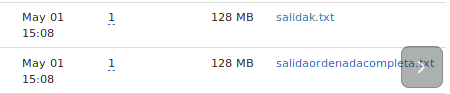
\includegraphics[width=.7\textwidth]{capitulo4a/images/corrida6.png}
		\caption{Archivos adicionales de salidas.}
		\label{fig:archivos}
	\end{center}
\end{figure}
El segundo archivo de salidas, es constituido por una salida ordenada del archivo, es decir, la misma información desplegada en \ref{fig:contenido} pero en este caso en orden ascendente de acuerdo a la distancia como se puede visualizar en la figura \ref{fig:ordenado}
\begin{figure}[H]
	\begin{center}
		\hypertarget{fig:ordenado}{\hspace{1pt}}
		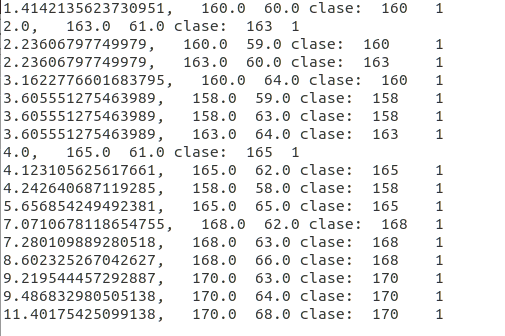
\includegraphics[width=.7\textwidth]{capitulo4a/images/ordenadacompleta.png}
		\caption{Archivo Salida Ordenada Completa.}
		\label{fig:ordenado}
	\end{center}
\end{figure}
En este archivo se puede visualizar la misma información que se presentaba anteriormente en el archivo \ref{fig:contenido} pero los datos están ordenados en forma ascendente por la distancia calculada. lo cual ya nos empieza a proporcionar una idea de cuales podrían ser los vecinos mas cercanos. \\
El ultimo archivo representa la salida final, como tal este únicamente muestra la cantidad de vecinos especificados y además de acuerdo a la clase seleccionada intenta clasificarlos siempre y cuando en el número de k seleccionado haya alguna clase para la que este número de elementos tenga más salidas. Lo anterior se muestra en la figura \ref{fig:salidak} 
\begin{figure}[H]
	\begin{center}
		\hypertarget{fig:salidak}{\hspace{1pt}}
		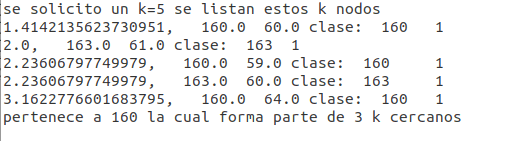
\includegraphics[width=.7\textwidth]{capitulo4a/images/kcercanos.png}
		\caption{Archivo Salida k.}
		\label{fig:salidak}
	\end{center}
\end{figure}
En este archivo, como se especificó un numero de vecinos igual a 5 entonces se muestran únicamente las primeras 5 entradas del archivo \ref{fig:ordenado} y ademas se busca la clase que como se puede ver se repite la clase \textbf{160} 3 veces en las 5 salidas por lo que se escribe que esta es la clase a la que pertenece con una cantidad de 3k vecinos cercanos.
\subsubsection{Prueba 2}
A continuación se muestra otra ejecución de este mismo algoritmo con diferentes configuraciones de properties para poder ver otra funcionalidad que puede ser aplicada al momento de hacer uso de este algoritmo. \\
El archivo de configuraciones escogido para esta ejecución, tiene la siguiente información:
\\
\begin{verbatim}
posicionescolumnas=2,3

buscar=S

elementoabuscar=62,L

origen= 161,61

posiciones=2,3

K=5
\end{verbatim}
Con estas configuraciones se indica:
\begin{itemize}
	\item Posicionescolumnas: Las columnas donde se encuentran los elementos que conforman la clase son la 2 y la 3. Es decir, para este ejemplo en particular, Peso y Talla
	\\
	\item Buscar: Al momento de indicar buscar en el valor de S significa que se tiene un determinado elemento en el valor de posiciones columnas el cual se desea buscar.\\
	Es decir, para valores diferentes de esta clase no se realizaría el análisis y se omitiría esa fila en el archivo 
	\item Elemento a Buscar: A continuación se muestra el elemento en particular que se desea buscar dentro del archivo. En este caso se indica que se trata del elemento 62,L.\\
	Cabe destacar que los elementos deben ser indicados tal cual se muestran en el archivo de datos de coma a coma, con los espacios y todo lo que venga incluido entre ellos. En caso de no realizarse de esta manera no se encontrarán coincidencias para estos elementos.
\end{itemize}
El archivo de entradas tiene la misma información para ser ocupada durante el proceso de análisis.
\\
Pero al momento de cambiar el archivo de configuración los resultados que podremos obtener serán diferentes.\\
\begin{verbatim}
Altura,Peso,Talla
160,60,M
163,61,M
160,59,M
163,60,M
160,64,L
158,59,M
158,63,M
163,64,L
165,61,L
165,62,L
158,58,M
165,65,L
168,62,L
168,63,L
168,66,L
170,63,L 
170,64,L 
170,68,L 
\end{verbatim}
A continuación se procede con la ejecución del algoritmo:
\\
esta se realiza con el comando siguiente:
\begin{verbatim}
root@maestro:/opt/hadoop/etc/hadoop: yarn jar /home/mayra/Escritorio/MRProgramsDemo.jar 
PackageDemo.WordCount "user/luminus/documentoknn1/tabla.txt" "user/luminus/documentoknn1/output1" "user/luminus/documentoknn1/configuracion.properties"
\end{verbatim} 
La ejecución de este algoritmo se puede ver en la figura \ref{fig:knn2ex}
\begin{figure}[H]
	\begin{center}
		\hypertarget{fig:knn2ex}{\hspace{1pt}}
		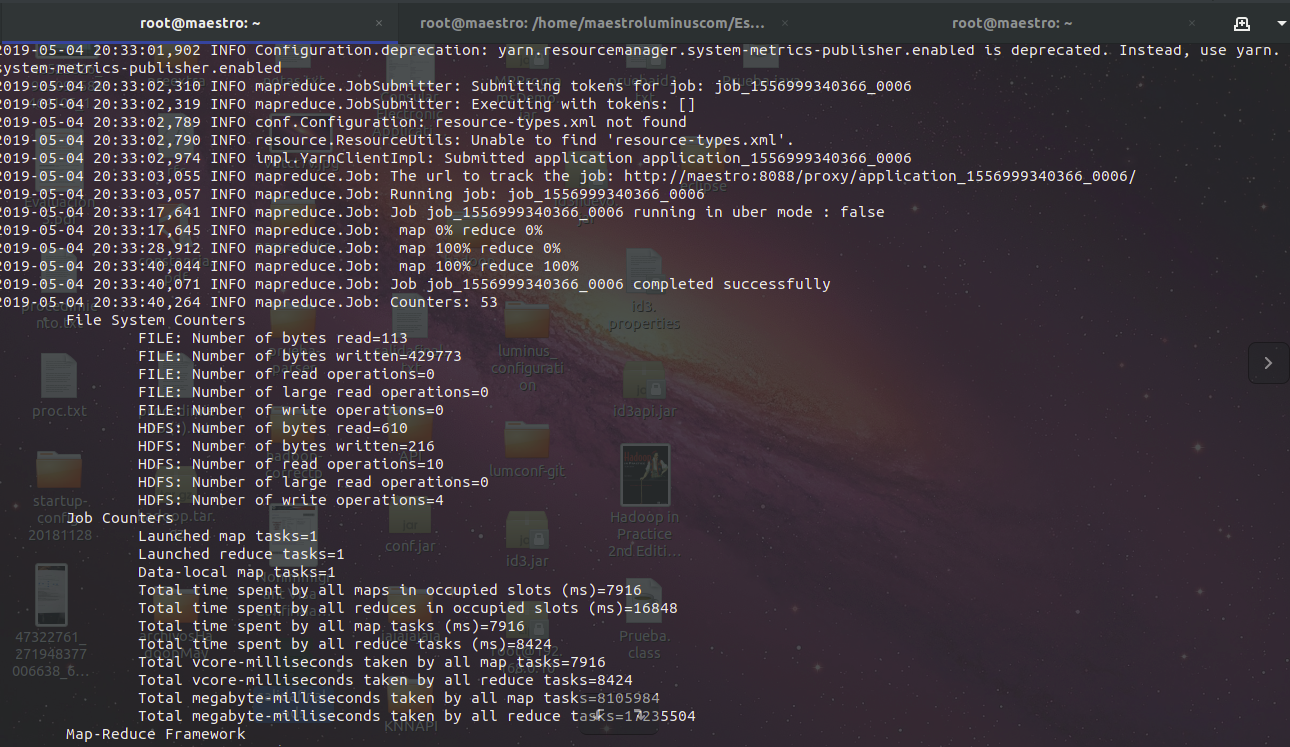
\includegraphics[width=.9\textwidth]{capitulo4a/images/ejecucionknn.png}
		\caption{Ejecución Algoritmo KNN.}
		\label{fig:knn2ex}
	\end{center}
\end{figure}
De primera instancia, como únicamente son evaluadas las entradas que contengan la información estipulada en el archivo de configuraciones, se tomarán en cuenta una cantidad inferior de entradas. \\
Por lo que el archivo de salidas completo se ve como se muestra en la figura \ref{fig:knn2ex1}
\begin{figure}[H]
	\begin{center}
		\hypertarget{fig:knn2ex1}{\hspace{1pt}}
		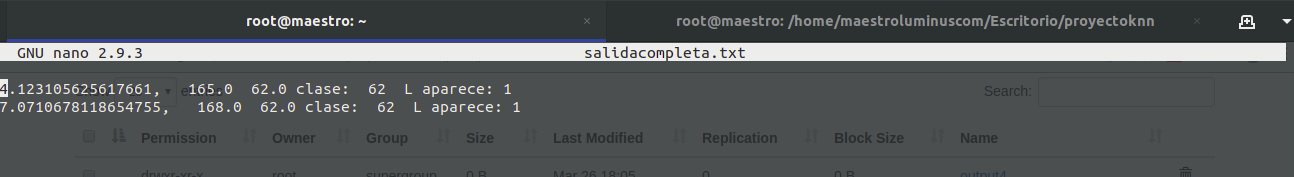
\includegraphics[width=.9\textwidth]{capitulo4a/images/salidacompleta.png}
		\caption{Salida completa algoritmo KNN.}
		\label{fig:knn2ex1}
	\end{center}
\end{figure}
Tomando entonces, esta salida como referencia, la salida ordenada completa se puede visualizar en la figura \ref{fig:knn2ex2}
\begin{figure}[H]
	\begin{center}
		\hypertarget{fig:knn2ex2}{\hspace{1pt}}
		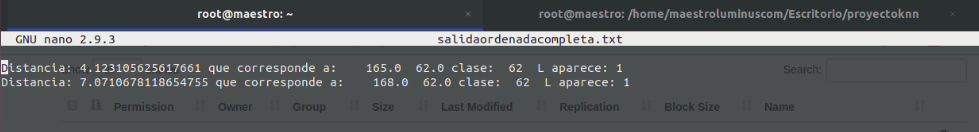
\includegraphics[width=.9\textwidth]{capitulo4a/images/salidaordenadacompleta.png}
		\caption{Salida Ordenada Completa KNN.}
		\label{fig:knn2ex2}
	\end{center}
\end{figure}
Una vez que se hace este ordenamiento, la siguiente salida es la salida K y se pidió una K igual a 5, pero como únicamente se pudieron obtener 2 k durante esta ejecución el algoritmo es persistente y de todas formas arroja la salida, únicamente mostrando las salidas que encontró, lo cual se puede ver en la figura \ref{fig:knn2ex3}.\\
\begin{figure}[H]
	\begin{center}
		\hypertarget{fig:knn2ex3}{\hspace{1pt}}
		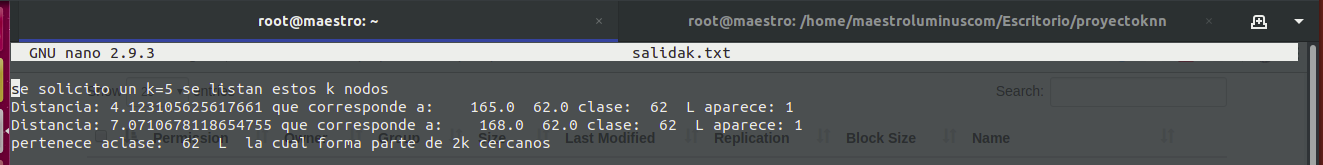
\includegraphics[width=.9\textwidth]{capitulo4a/images/salidak.png}
		\caption{Salida K algoritmo KNN}
		\label{fig:knn2ex3}
	\end{center}
\end{figure} 
Como se puede observar, debido a que la clase de las salidas es la misma, se clasifica el elemento en esta clase, y a pesar de que se pide un número de 5 nodos cercanos únicamente se muestran 2. 
\\
Por otro lado, se genera esta salida también en tipo excel, la cual se muestra a continuación en la siguiente figura \ref{fig:knn2ex4}:
\begin{figure}[H]
	\begin{center}
		\hypertarget{fig:knn2ex4}{\hspace{1pt}}
		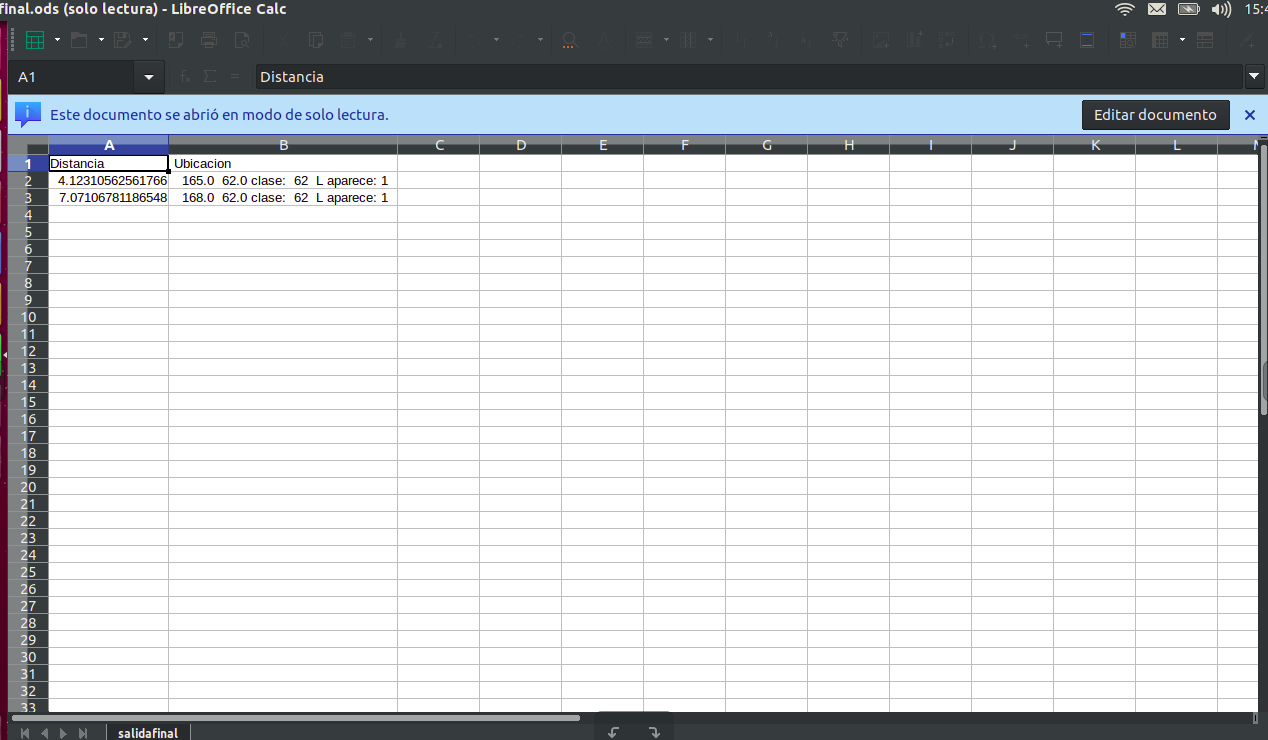
\includegraphics[width=.9\textwidth]{capitulo4a/images/salidaexcel.png}
		\caption{Salida en formato Excel Algoritmo KNN.}
		\label{fig:knn2ex4}
	\end{center}
\end{figure} 
Con esto, se podrían dar por concluidas las pruebas del algoritmo KNN, con lo que se puede decir que este opera de manera correcta con y sin el uso de la característica extra de agrupación por clase y las pruebas han resultado exitosas.
\subsection{Algoritmo ID3}
A continuación se muestra una prueba de la ejecución de este algoritmo para comprobar su correcto funcionamiento y que esta operando como debería hacerlo:
\\
Para ello y con el objetivo de que sea mas claro, se utilizará el mismo ejemplo que fue revisado en el marco teórico del presente documento, el cual puede ser visualizado en \nameref{ejecucionID3}.
\\
Esto debido a que se trata de un ejemplo el cual, ya es conocido y se conoce la forma en la que debe operar y los resultados esperados por lo que en este sentido facilitará el entendimiento de la prueba. 
\\
Como primer instancia es necesario crear el archivo de configuraciones para esta ejecución, el cual deberá contener la siguiente información:
\begin{verbatim}
posicionresultado=4

opciones=N,P

nombres=General,Temperatura,Humedad,Viento,Clase
\end{verbatim} 
Además, se procede a crear el archivo de entradas el cual contiene la información que será necesaria para la ejecución del algoritmo este archivo de entradas es el siguiente:
\begin{verbatim}
Soleado,caliente,alta,no,N

soleado,caliente,alta,si,N

nublado,caliente,alta,no,P

lluvioso,templada,alta,no,P

lluvioso,fria,normal,no,P

lluvioso,fria,normal,si,N

nublado,fria,normal,si,P

soleado,templada,alta,no,N

soleado,fria,normal,no,P

lluvioso,templada,normal,no,P

soleado,templada,normal,si,P

nublado,templada,alta,si,P

nublado,caliente,normal,no,P

lluvioso,templada,alta,si,N
\end{verbatim} 
Una vez listas estas configuraciones iniciales se procede a iniciar la ejecución de este algoritmo esto haciendo uso de la siguiente instrucción de línea de comandos.
 \begin{verbatim}
root@maestro:/opt/hadoop/etc/hadoop: yarn jar /home/mayra/Escritorio/ID3.jar 
id3.id3algoritm "user/luminus/ID3/pruebaid3.txt" "user/luminus/ID3/salidaid3Documento" "user/luminus/ID3/id3.properties"
\end{verbatim} 
La segunda especificada es la ruta dentro de la cual se escribirá la primera salida de la ejecución.\\
Es importante resaltar que una vez que termine de ejecutar el primer job se buscará la siguiente carpeta donde continuará escribiendo los resultados, por lo que se tiene que destinar una carpeta donde se escribirán el resto de salidas. la información relacionada con esta carpeta será introducida desde la interface de programación de aplicaciones de Luminus que hará uso de este algoritmo, y la escribirá directamente sobre el archivo properties.
En la figura \ref{fig:ID31} se puede apreciar la puesta en marcha y el inicio de ejecución de este algoritmo.\\
\begin{figure}[H]
	\begin{center}
		\hypertarget{fig:ID31}{\hspace{1pt}}
		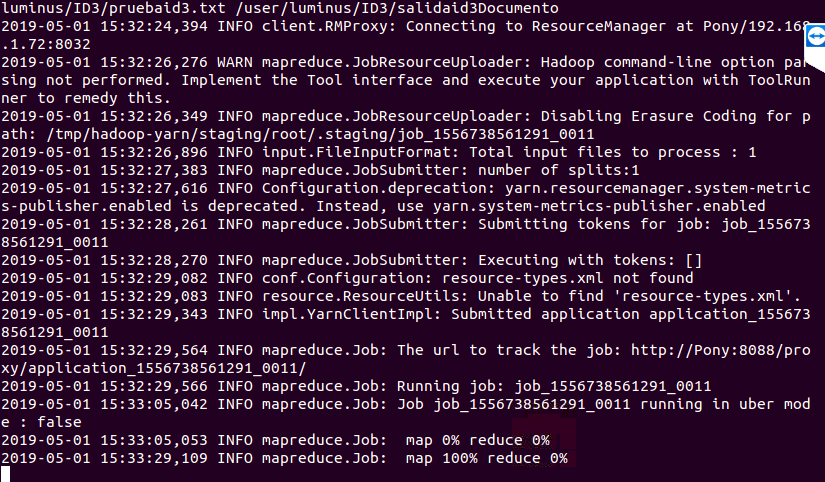
\includegraphics[width=.7\textwidth]{capitulo4a/images/ID3_1.png}
		\caption{Primera corrida del algoritmo ID3.}
		\label{fig:ID31}
	\end{center}
\end{figure}
Posteriomente, cuando esta primera ejecución finalice nos dará un resultado parcial de la salida de la primera ejecución la cual para este tipo de corrida puede ser visualizada desde pantalla, como se muestra en la figura \ref{fig:ID34} los cálculos intermedios y las escrituras de la salida de este job pueden ser visualizadas en las imágenes \ref{fig:ID32} y \ref{fig:ID33}. 
\begin{figure}[H]
	\begin{center}
		\hypertarget{fig:ID32}{\hspace{1pt}}
		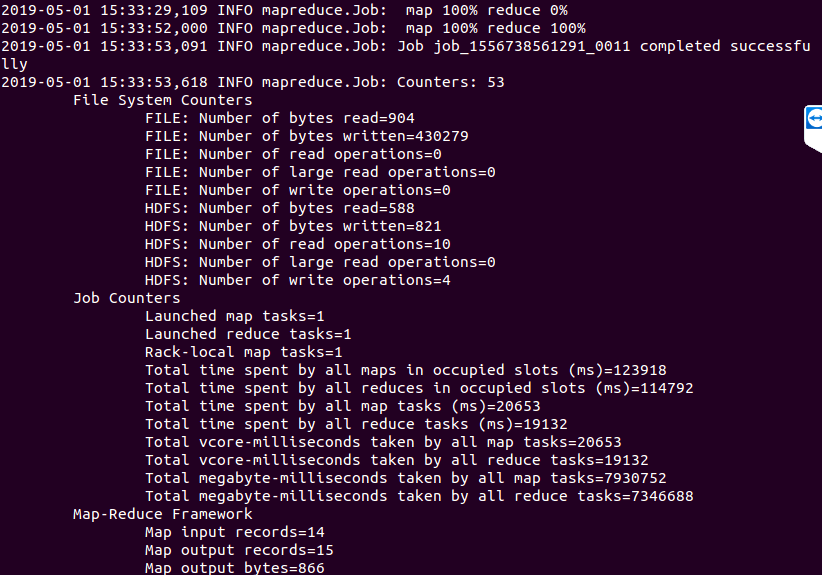
\includegraphics[width=.7\textwidth]{capitulo4a/images/ID3_2.png}
		\caption{Pasos intermedios de la ejecución.}
		\label{fig:ID32}
	\end{center}
\end{figure}
\begin{figure}[H]
	\begin{center}
		\hypertarget{fig:ID33}{\hspace{1pt}}
		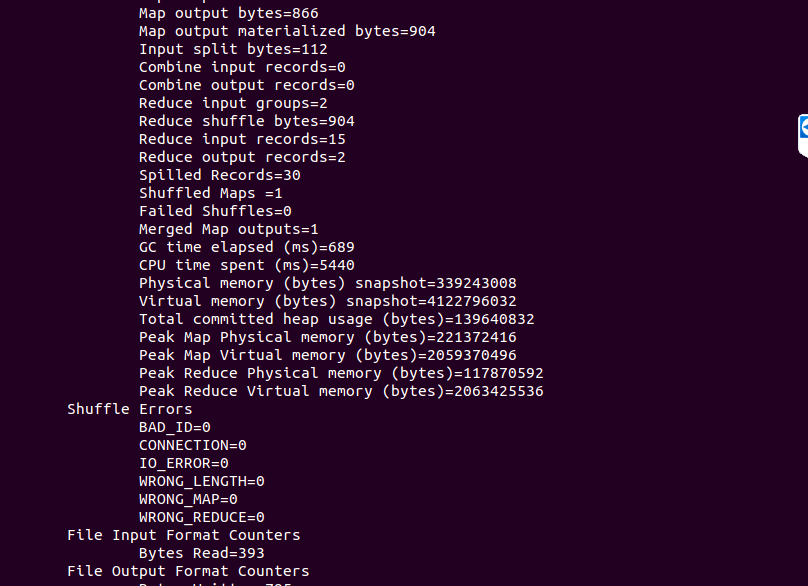
\includegraphics[width=.7\textwidth]{capitulo4a/images/ID3_3.png}
		\caption{Pasos intermedios de la ejecución.}
		\label{fig:ID33}
	\end{center}
\end{figure} 
\begin{figure}[H]
	\begin{center}
		\hypertarget{fig:ID31}{\hspace{1pt}}
		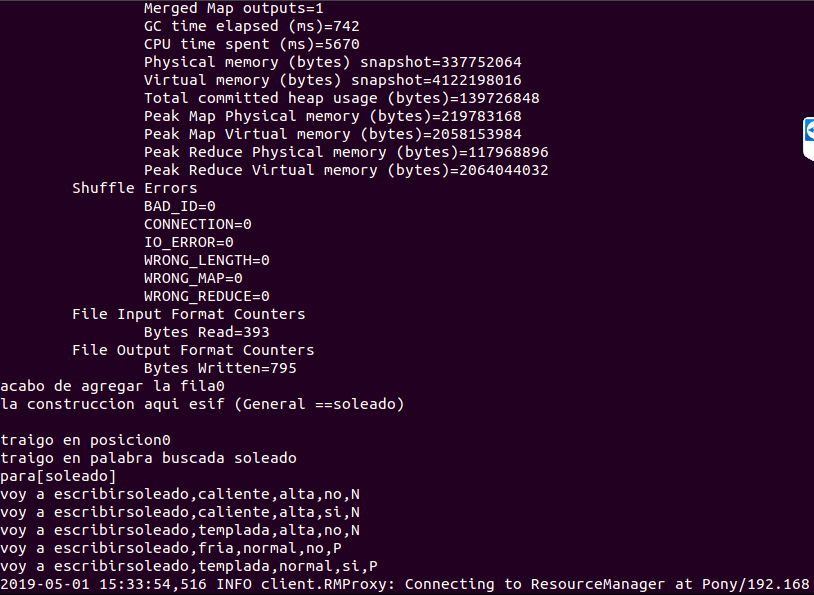
\includegraphics[width=.7\textwidth]{capitulo4a/images/ID3_4.png}
		\caption{Primera corrida del algoritmo ID3.}
		\label{fig:ID34}
	\end{center}
\end{figure}
por lo que una vez que se obtiene el primer resultado parcial se procede a la ejecución de los subsecuentes jobs de trabajo, estos se irán levantando uno a uno conforme vaya finalizando el anterior, cada vez que uno de estos finalice será posible visualizar su salida intermedia y con esto permitir que el job subsecuente inicie su ejecución estos resultados parciales de los que se habla se pueden visualizar en las figuras \ref{fig:ID35},\ref{fig:ID36},\ref{fig:ID37},\ref{fig:ID38},\ref{fig:ID39}y \ref{fig:ID310}. para cada una de ellas es posible visualizar la salida intermedia que se tenia en ese momento de la ejecución, la nueva inicialización del nuevo job para continuar y el detalle en el pie de imagen de que combinación de columnas se estaba evaluando en ese momento. \\
Con lo que con las figuras presentadas se puede dar seguimiento a la evolución de la ejecución y como es que esta ejecución se va comportando con respecto a la recursividad. 
\begin{figure}[H]
	\begin{center}
		\hypertarget{fig:ID35}{\hspace{1pt}}
		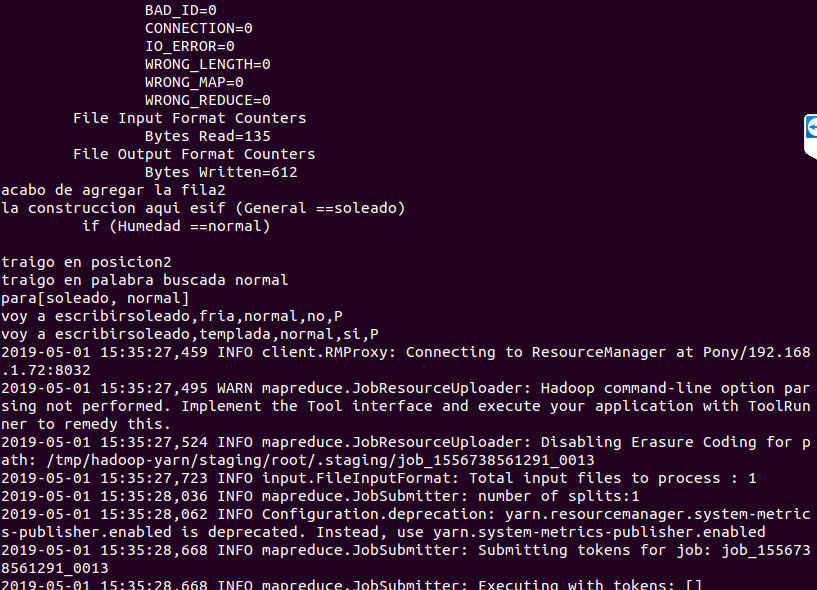
\includegraphics[width=.7\textwidth]{capitulo4a/images/ID3_6.png}
		\caption{Salidas intermedias para Soleado-Normal.}
		\label{fig:ID35}
	\end{center}
\end{figure}
\begin{figure}[H]
	\begin{center}
		\hypertarget{fig:ID36}{\hspace{1pt}}
		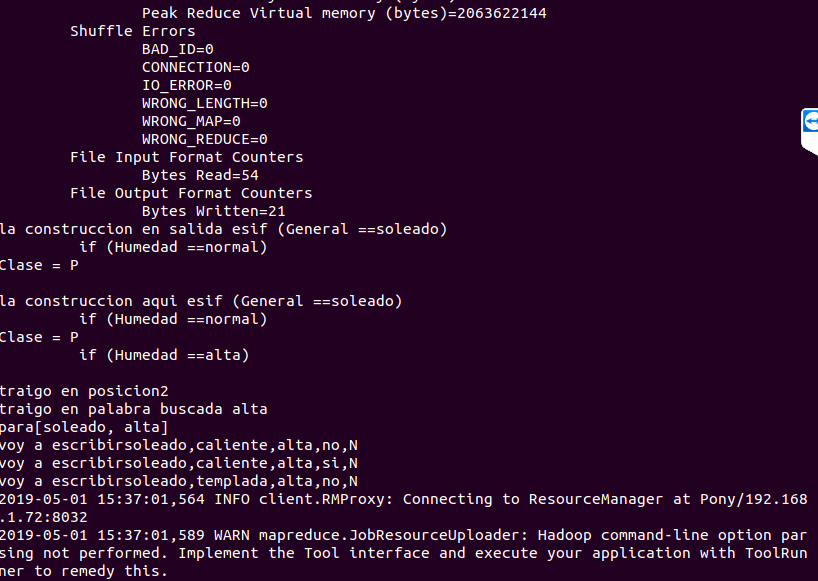
\includegraphics[width=.7\textwidth]{capitulo4a/images/ID3_8.png}
		\caption{Salidas intermedias para Soleado-Alta.}
		\label{fig:ID36}
	\end{center}
\end{figure}
\begin{figure}[H]
	\begin{center}
		\hypertarget{fig:ID37}{\hspace{1pt}}
		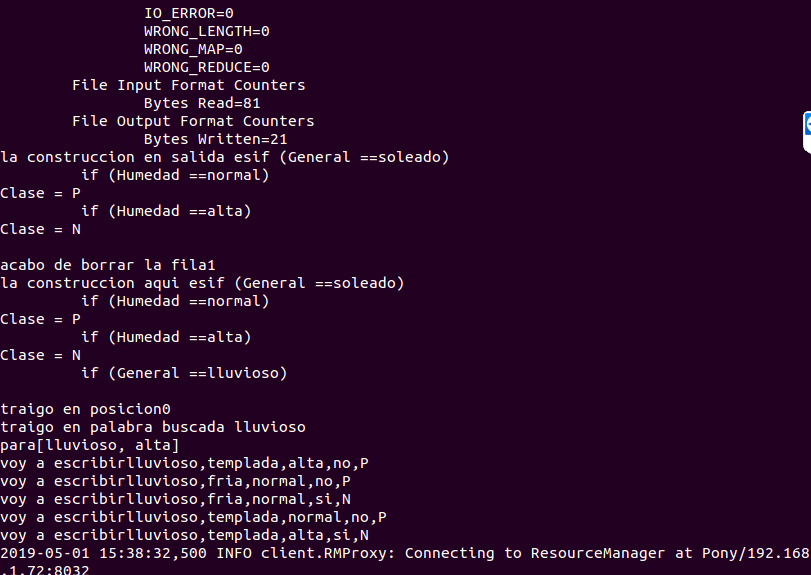
\includegraphics[width=.7\textwidth]{capitulo4a/images/ID3_9.png}
		\caption{Salidas intermedias para Lluvioso.}
		\label{fig:ID37}
	\end{center}
\end{figure}
\begin{figure}[H]
	\begin{center}
		\hypertarget{fig:ID38}{\hspace{1pt}}
		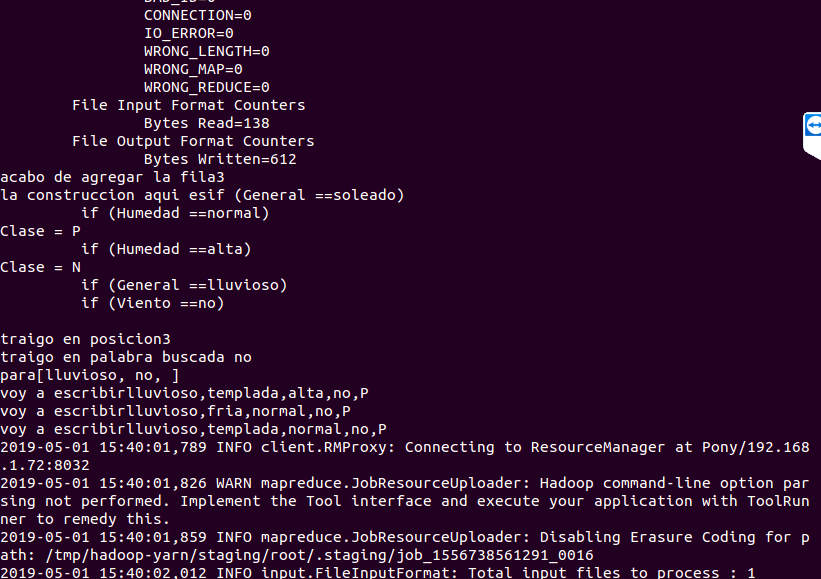
\includegraphics[width=.7\textwidth]{capitulo4a/images/ID3_10.png}
		\caption{Salidas intermedias para Lluvioso-No.}
		\label{fig:ID38}
	\end{center}
\end{figure}
\begin{figure}[H]
	\begin{center}
		\hypertarget{fig:ID39}{\hspace{1pt}}
		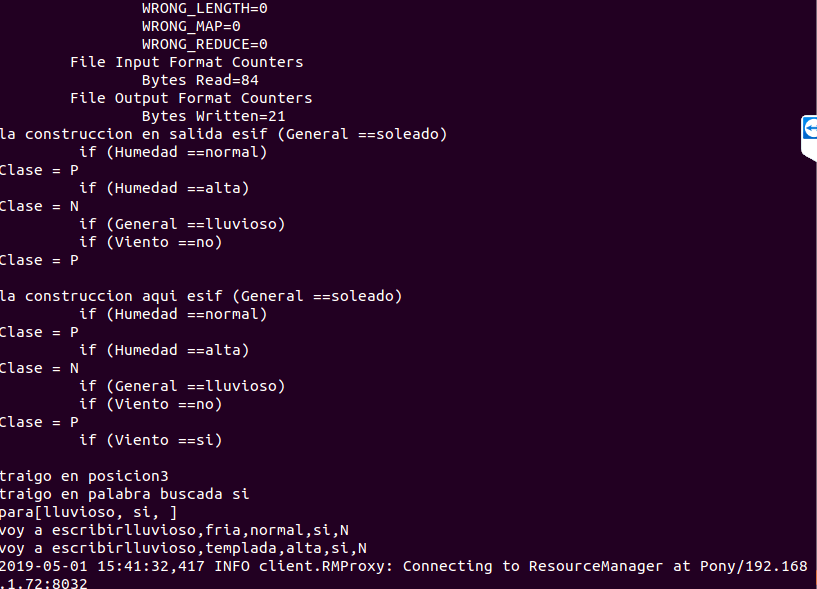
\includegraphics[width=.7\textwidth]{capitulo4a/images/ID3_12.png}
		\caption{Salidas intermedias para Lluvioso-Si.}
		\label{fig:ID39}
	\end{center}
\end{figure}
\begin{figure}[H]
	\begin{center}
		\hypertarget{fig:ID310}{\hspace{1pt}}
		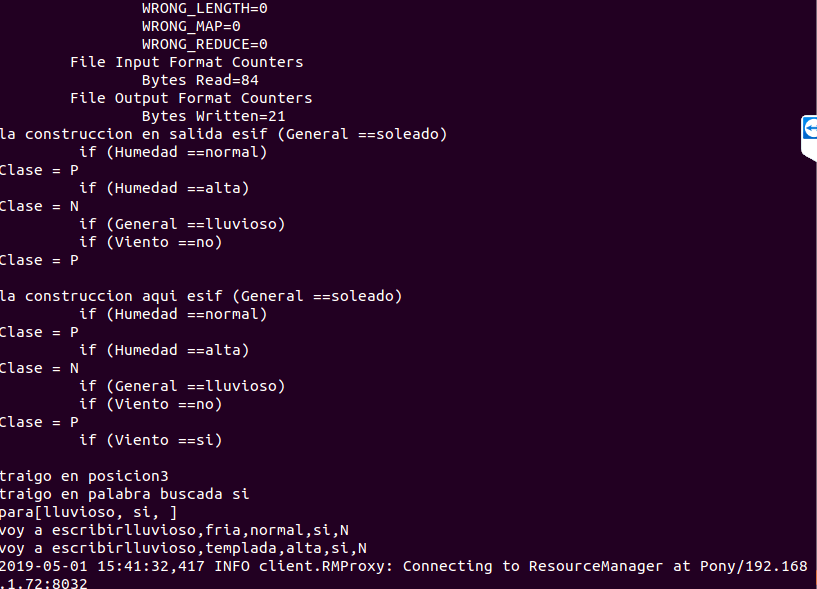
\includegraphics[width=.7\textwidth]{capitulo4a/images/ID3_12.png}
		\caption{Salidas intermedias para Nublado.}
		\label{fig:ID310}
	\end{center}
\end{figure}
Al finalizar todos los puntos intermedios, finalmente se puede llegar a la última ejecución la cual finaliza el proceso y termina, esto es cuando termina de realizar todas las evaluaciones de todas las columnas obtenidas durante la función recursiva. 
\\
Debido a que cada que llega una nueva columna se va a agregando a un arreglo de columnas, y cada que una columna termina de ser evaluada en su totalidad esta se elimina del arreglo de columnas, cuando la última fila de este arreglo es eliminada es decir, la fila 0. 
Quiere decir que la ejecución termino exitosamente como se puede observar en la figura \ref{fig:ID311} donde se puede ver que ya se imprime la salida final para este ejemplo y además se puede visualizar como se elimina la fila 0.
\begin{figure}[H]
	\begin{center}
		\hypertarget{fig:ID310}{\hspace{1pt}}
		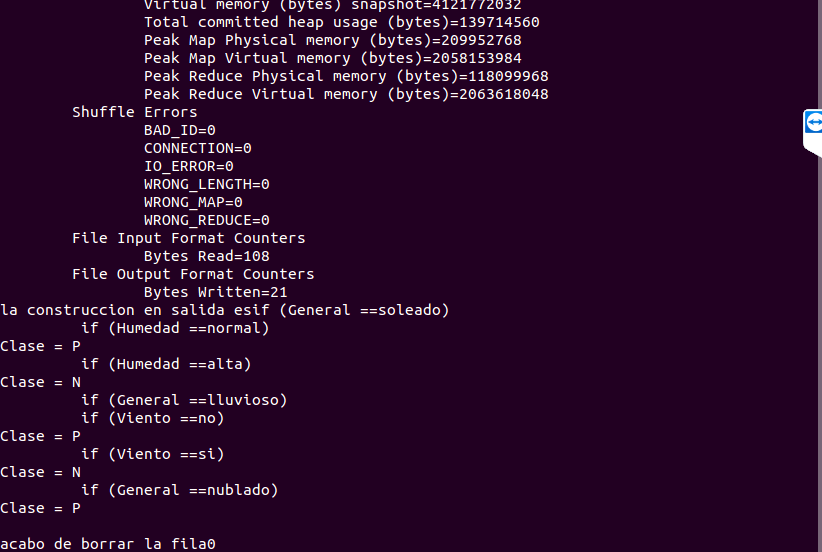
\includegraphics[width=.7\textwidth]{capitulo4a/images/ID3_15.png}
		\caption{Finaliza Ejecución de algoritmo ID3}
		\label{fig:ID311}
	\end{center}
\end{figure}
Cuando la ejecución termina, entonces se puede visualizar el archivo de salidas establecido para la ejecución en el HDFS como se muestra en la figura \ref{fig:ID312}, cabe señalar, que este archivo únicamente contiene la información de la primera ejecución de MapReduce debido a que cada ejecución requiere un nuevo directorio de salidas.
\begin{figure}[H]
	\begin{center}
		\hypertarget{fig:ID312}{\hspace{1pt}}
		
\includegraphics[width=.7\textwidth]{capitulo4a/images/ID3_17.png}
		\caption{Visualización de archivo de salidas de linea de comandos(Primera ejecución en el HDFS)}
		\label{fig:ID312}
	\end{center}
\end{figure}
Sin embargo, si se procede a visualizar el interior de este directorio en el archivo \emph{part-00000} se encuentra la información contenida en la figura \ref{fig:ID313} la cual contiene toda la información relacionada con la primera corrida, se puede visualizar los cálculos de las entropías y las ganancias realizados y finalmente se puede conocer la fila que se determinó con la mayor ganancia y los elemento que esta fila contiene.
\begin{figure}[H]
	\begin{center}
		\hypertarget{fig:ID313}{\hspace{1pt}}
		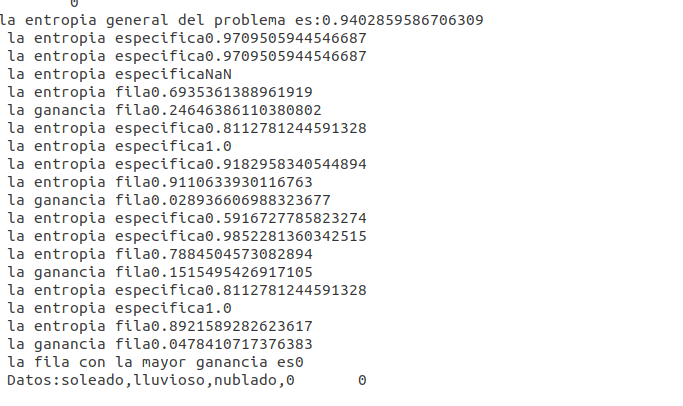
\includegraphics[width=.7\textwidth]{capitulo4a/images/ID3_18.png}
		\caption{Salida del archivo Part-00000}
		\label{fig:ID313}
	\end{center}
\end{figure}
Sin embargo, esta no constituye la totalidad de la ejecución del algoritmo ya que como se mencionaba cada ejecución genera su propia carpeta de salida. 
\\
Para este caso en particular, la ruta donde estos directorios fueron escritos es:
\begin{verbatim}
/user/luminus/ID3/pruebasjob
\end{verbatim} 
La información contenida en este directorio puede ser visualizada en la figura \ref{fig:ID314}
\begin{figure}[H]
	\begin{center}
		\hypertarget{fig:ID313}{\hspace{1pt}}
		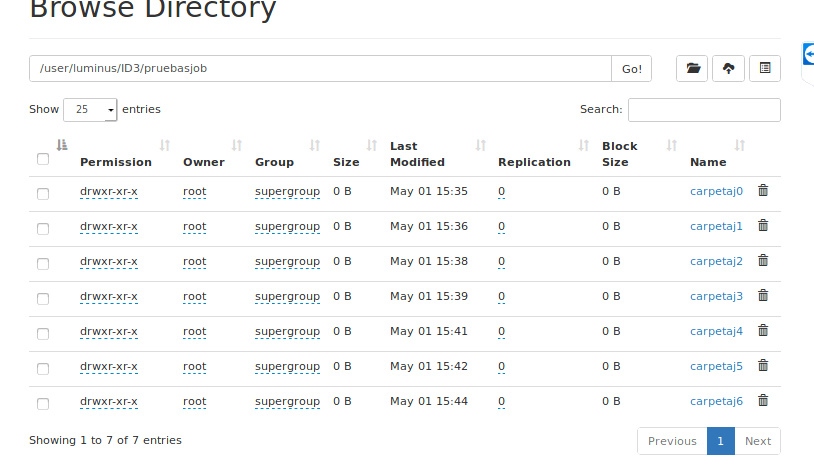
\includegraphics[width=.7\textwidth]{capitulo4a/images/ID3_19.png}
		\caption{Directorio de salidas de HDFS para trabajos posteriores}
		\label{fig:ID314}
	\end{center}
\end{figure}
Siguiendo la misma lógica de funcionamiento esperada para el primer directorio, se procede a visualizar la información de salida contenida en cada uno de los directorios y se dará una breve información del porque se presenta esta información. \\
La primera salida se muestra en la figura \ref{fig:ID315} esta corresponde al cálculo de ganancias y entropias que dan como resultado la fila con mayor ganancia 2. \\
Esto ocurre cuando se ejecuta el algoritmo tomando en cuenta únicamente las entradas de la tabla donde en la columna 0 poseen el valor de soleado.\\
Como se requiere aproximar un poco más y probar con una nueva fila, se realiza entonces este cálculo.
\begin{figure}[H]
	\begin{center}
		\hypertarget{fig:ID315}{\hspace{1pt}}
		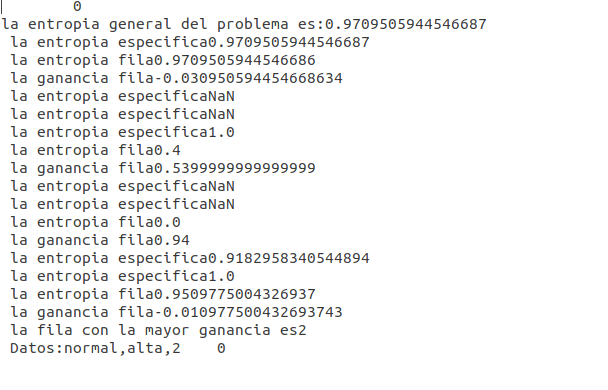
\includegraphics[width=.7\textwidth]{capitulo4a/images/ID3_20.png}
		\caption{Salida de carpetaj0}
		\label{fig:ID315}
	\end{center}
\end{figure}
La salida subsecuente se muestra en la figura \ref{fig:ID316}. Y debido a que se establece que Soleado y Normal, esto es todo lo que se necesita para hacer una clasificación entonces se llega a un caso base y únicamente se indica en este archivo.
\begin{figure}[H]
	\begin{center}
		\hypertarget{fig:ID316}{\hspace{1pt}}
		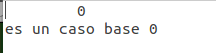
\includegraphics[width=.3\textwidth]{capitulo4a/images/ID3_21.png}
		\caption{Salida de carpetaj1}
		\label{fig:ID316}
	\end{center}
\end{figure}
La siguiente salida se muestra en la figura \ref{fig:ID317}. Esta también constituye un caso base y esto se debe a una situación muy parecida a la de la figura \ref{fig:ID316} ya que en este caso Soleado y Alta también constituyen un caso base. 
\begin{figure}[H]
	\begin{center}
		\hypertarget{fig:ID317}{\hspace{1pt}}
		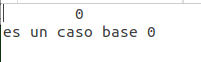
\includegraphics[width=.3\textwidth]{capitulo4a/images/ID3_22.png}
		\caption{Salida de carpetaj2}
		\label{fig:ID317}
	\end{center}
\end{figure}
Para la siguiente ejecución se procede a trabajar con Lluvioso, el cual únicamente de esta forma no genera un caso pase por lo que se procede a realizar nuevamente los cálculos pertinentes para obtener una nueva columna a evaluar, de acuerdo a la figura \ref{fig:ID318} se puede ver que se obtiene que la fila con mayor ganancia es la 3 y que los valores que esta fila contiene es NO y SI.
\begin{figure}[H]
	\begin{center}
		\hypertarget{fig:ID318}{\hspace{1pt}}
		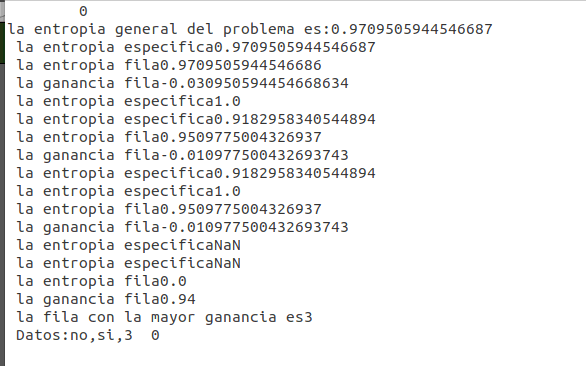
\includegraphics[width=.7\textwidth]{capitulo4a/images/ID3_23.png}
		\caption{Salida de carpetaj3}
		\label{fig:ID318}
	\end{center}
\end{figure}
Debido a que la respuesta final para la siguiente evaluación es Lluvioso- No, entonces no se requiere realizar nuevamente el cálculo de ganancias y entropías por lo que el siguiente archivo el cual se muestra en la figura \ref{fig:ID319} representa un caso base.
\begin{figure}[H]
	\begin{center}
		\hypertarget{fig:ID319}{\hspace{1pt}}
		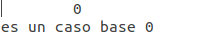
\includegraphics[width=.3\textwidth]{capitulo4a/images/ID3_24.png}
		\caption{Salida de carpetaj4}
		\label{fig:ID319}
	\end{center}
\end{figure}
Un caso muy similar ocurre con la siguiente entrada y el siguiente archivo el cual se muestra en la figura \ref{fig:ID320} debido a que Lluvioso- Si representa un caso base, la información descrita en este archivo describe ese detalle. 
\begin{figure}[H]
	\begin{center}
		\hypertarget{fig:ID320}{\hspace{1pt}}
		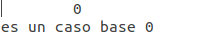
\includegraphics[width=.3\textwidth]{capitulo4a/images/ID3_24.png}
		\caption{Salida de carpetaj5}
		\label{fig:ID320}
	\end{center}
\end{figure}
Una vez que se termina de efectuar la evaluación correspondiente a la columna 3, esta se retira del listado de columnas y se regresa a la columna 0, debido a que en la columna 0 aun se encuentra el valor de Nublado, se procede a realizar la evaluación de este valor, sin embargo desde este momento ya se trata de un elemento clasificado por lo que, se trata de un caso base como se muestra en la figura \ref{fig:ID321}.
 \begin{figure}[H]
 	\begin{center}
 		\hypertarget{fig:ID321}{\hspace{1pt}}
 		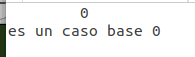
\includegraphics[width=.3\textwidth]{capitulo4a/images/ID3_27.png}
 		\caption{Salida de carpetaj6}
 		\label{fig:ID321}
 	\end{center}
 \end{figure}
 Como último paso se procede a presentar en la figura \ref{fig:ID322} el archivo final de salidas para la ejecución de este algoritmo. 
  \begin{figure}[H]
  	\begin{center}
  		\hypertarget{fig:ID322}{\hspace{1pt}}
  		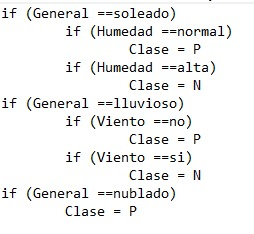
\includegraphics[width=.5\textwidth]{capitulo4a/images/ID3_FINAL.png}
  		\caption{Salida final del algoritmo ID3 para este ejemplo}
  		\label{fig:ID322}
  	\end{center}
  \end{figure}
 La cual contiene la información, que se despliega desde línea de comandos presentada en la figura \ref{fig:ID311} pero ya en un archivo permanente para consulta y uso por parte del usuario final. 
 Se encuentra con las identaciones correspondientes para que se comprenda a que nivel corresponde cada columna evaluada.
 Con esto se puede afirmar que los cálculos se llevaron a cabo de manera exitosa y que el algoritmo ID3 funciona correctamente.